\documentclass[bibliography=totoc,liststotoc,BCOR5mm,DIV12,oneside,headlines=2]{scrbook}

% use this declaration to set specific page margins
%\usepackage[a4paper , lmargin = {3.5cm} , rmargin = {2.7cm} , tmargin = {2.7cm} , bmargin = {4.6cm} ]{geometry}
\usepackage[a4paper]{geometry}

\usepackage[ngerman, english]{babel}
\usepackage{bibgerm}       		% german references
\usepackage[utf8]{inputenc} % german characters
% it's recommended to use PDF images but you can use JPG or PNG as well
\usepackage{graphicx}
\usepackage{url}           		% format URLs
\usepackage{hyperref} 				% create hyperlinks
\usepackage{listings, color}	% for source code
\usepackage{subfig}						% two figures next to each other (example: figure 3a), figure 3b)
\usepackage{scrpage2}					% header and footer line

% header and footer line - no header & footer line on pages where a new chapter starts
\clearscrheadfoot
\pagestyle{scrheadings}
\ohead{Framework design for automated feature extraction\\ from semi-structured information entities}
\ihead{Peter Schrott}
\setheadsepline{0.2pt}
\ofoot[]{\thepage}
\ifoot{Master Thesis, TU Berlin, Chair of IKM, 2017}

% set path where images are stored
\graphicspath{{./img/}}

%
% der Befehl \hypenation versteht keine Sonderzeichen, also weder ä
% noch "a noch \"a. Wörter die derartige Zeichen enthalten müssen
% direkt im Text getrennt werden, z.B. Wör\-ter
%
\hyphenation{te-le-com-muni-cation 
te-le-com-muni-cation-specific 
Te-le-kom-mu-ni-ka-tions-API} 					% use this file to set explicit hyphenations (doesn't seem to work correctly)

% "define" Scala
\usepackage[T1]{fontenc}
\usepackage{beramono}
\usepackage{listings}
\usepackage{xcolor}

\definecolor{dkgreen}{rgb}{0,0.6,0}
\definecolor{gray}{rgb}{0.5,0.5,0.5}
\definecolor{mauve}{rgb}{0.58,0,0.82}

\lstdefinestyle{myScalastyle}{
  frame=tb,
  language=scala,
  aboveskip=3mm,
  belowskip=3mm,
  showstringspaces=false,
  columns=flexible,
  basicstyle={\small\ttfamily},
  numbers=none,
  numberstyle=\tiny\color{gray},
  keywordstyle=\color{blue},
  commentstyle=\color{dkgreen},
  stringstyle=\color{mauve},
  frame=single,
  breaklines=true,
  breakatwhitespace=true,
  tabsize=3,
}

\begin{document}
% ---------------------------------------------------------------
\frontmatter
    \thispagestyle{empty}
\begin{center}

\vspace*{1.2cm}
{\LARGE \textbf{Technische Universität Berlin}}

\vspace{0.5cm}

%{\large Institut für Telekommunikationssysteme\\[1mm]}
{\large Chair of Information and Communication Management (IKM)\\[5mm]}

Fakultät VII\\
Straße des 17. Juni 135\\
10623 Berlin\\

\vspace*{1cm}


\includegraphics[width=4cm]{tu_logo.jpg}

\vspace*{1.0cm}

{\large Master Thesis}\\

\vspace{1.0cm}
{\LARGE \textbf{Framework design for automated}}\\
\vspace*{0.25cm}
{\LARGE \textbf{feature extraction from semi-structured}}\\
\vspace*{0.35cm}
{\LARGE \textbf{ information entities}}\\
\vspace*{1.0cm}
{\LARGE Peter Schrott}
\\
\vspace*{0.5cm}
Matriculation Number: 370314\\
24.07.2017\\ % 	date of submission
\vspace*{1.0cm}

Supervised by\\
Prof. Dr. Rüdiger Zarnekow\\
\vspace*{0.5cm}
Secondary Supervisor\\
Prof. Dr. rer. nat. Volker Markl
\vspace{3cm}

\end{center}
   	\thispagestyle{empty}
    \cleardoublepage 
    
    \thispagestyle{empty}
\vspace*{3cm}

\vspace*{1cm}
\noindent 
First of all I would like to thank Prof. Dr. Rüdiger Zarnekow at the Chair of Communication and Information Management for giving me the opportunity to carry out state of the art research in this field. As a joint venture thesis in in the field of computer science and communication and information management this thesis shows the necessity of knowledge exchange over organizational boundaries. The introduction of aspects going further then sheer technical views widened my horizon and resulted in a great and reusable result of this work. 
\\
\\
Special thanks to Hannes Kübel for his guidance throughout the duration of this master thesis. His tutor abilities from the first idea sketch until the final commitment of the topic is more than mentionable. Unfortunately Hannes had to leave me during the writing of my thesis due to the finishing of his dissertation. For that reason I also like to thank XY for the smooth take over and further professional mentoring.
\\
\\
Furthermore I want to thank my family and friends, standing with me and supporting me personally trough the long period of the thesis. Not turning their back on me after silence from my side for several weeks and having an open ear on and understanding attitude. I will never forget this kind of personal backing.
    \thispagestyle{empty}
    \cleardoublepage
    
    \newpage

\thispagestyle{empty}

\begin{large}

\vspace*{6cm}

\noindent
Hereby I declare that I wrote this thesis myself with the help of no more than the mentioned literature and auxiliary means.
\vspace{2cm}

\noindent
Berlin, 25.07.2017

\vspace{3cm}

\hspace*{7cm}%
\dotfill\\
\hspace*{8.5cm}%
\textit{(Signature Peter Schrott)}

\end{large}
 
    \thispagestyle{empty}
    \cleardoublepage
    
    \thispagestyle{empty}
\vspace*{1.0cm}

\begin{center}
    \textbf{Abstract}
\end{center}

\vspace*{0.5cm}

\noindent
The thesis is about to introduce a framework that automates the feature extraction from semi-structured information entities. In a world of a ever growing amount of data digitally available their diversity is reaching unprecedented levels. Instances exist that highly depend on the quality of input data but also require a broad mass of information. For appropriate and most beneficial usage of data that are aggregated across several sources it is essential to find a unified representation to satisfy an applications demand for data purity. The initial focus of this work lies on the structuring of the problems of distributed and messy data. A breakdown of the wide spectrum of issues results in a a concrete and generalized categorization of data problems.  This categorization proofs to be aligned with modern data storage technologies as well as well established and aged storage approaches. The analysis provides a solid bases for the rest of the work. Irrespective of underlying systems, data formats or structures, the scope and target is defined. 

In a problem driven approach the initial data issue categorization is used to define the requirements for novel framework handling heterogeneous data with the aim of transforming them into valuable representations. The requirements are related to technical as well as economical aspects and set the fundamentals for a intuitive concept. In the focus is the automation and the extendability of the final solution. With the outlook for a reference implementation a pragmatic concept is defined. Here a modularized approach is chosen to generate the most possible coverage of the beforehand stated demands. The requirement engineering as well as the concept finding has a strong focus of the problem environment and is detached from technical details. Through an reference implementation the concept is challenged with respect to the elaborated requirements. Questions regarding technical foundations, libraries and frameworks are addressed. A clean technical concept is found and a intuitive abstraction of the underlying problem is set up. 

A comprehensive evaluation points out the applicability and realizability of the proposed framework and shows the success of the problem driven approach. Furthermore the majority of the evaluation is devoted to the assessment of the systems learning ability. Under this point a toy dataset is introduced that measures the performance while it proves the frameworks readiness to use. The final conclusion summarizes this work and assesses the use of the framework through an overall viewpoint. After presenting encounter problems a lookout for further work is given.
    \thispagestyle{empty}
    \cleardoublepage
    
    %\thispagestyle{empty}
\vspace*{0.2cm}

\begin{center}
    \textbf{Zusammenfassung}
\end{center}

\vspace*{0.2cm}

\noindent 
Da die meisten Leuten an der TU deutsch als Muttersprache haben, empfiehlt es sich, das Abstract zusätzlich auch in deutsch zu schreiben. Man kann es auch nur auf deutsch schreiben und anschließend einem Englisch-Muttersprachler zur Übersetzung geben.
    %\thispagestyle{empty}
    
    \tableofcontents
    \thispagestyle{empty}
    
    \listoffigures
    \thispagestyle{empty}
    
    \listoftables
    \thispagestyle{empty}
    
% --------------------------------------------------------------

\mainmatter % comment single chapters for faster compilation

    \chapter{Introduction\label{cha:chapter1}}

"Oder in the chaos and chaos in the order", is is how Osterhold\cite[p. 24f]{osterhold_2013} describes one of the two essential research directions of chaos theory. Furthermore she claims, "processes, procedures or structures that appear very disordered only prove to be chaotic prior to the point they are analyzed further". This generalized and theoretical approach can be directly transfered to computer science, especially the field of information retrieval, data mining and data processing. 

\section{Motivation\label{sec:moti}}

The todays unbounded growth of information digitally available suggests a massive and chaotic collection of data. An in 2014 published report by ICD states that the digitalized data grow by 100\% every two years and will reach 44 zettabytes (10\textsuperscript{21} bytes) by 2020 - as many stars as known in the universe\cite{data_growth_2014}.
\\\\
Data in general, but also massive amounts of data, are only of value if they are utilized appropriately. Gaining deeper insights is the point of data transformation, data visualization or calculations on data. From a technical as well as an economical point of view a high degree of automation in data processing is required for maximizing the efficiency, especially when it comes to handling a high number of information entities\cite{labrinidis_jagadish_2012}. A large variety of software solutions is available that enable automated data processing for numerous domains and complexity levels. The solutions capture all levels of abstraction and reach from end user desktop applications, e.g. Microsoft Excel\cite{excel_2017}, for the daily use, to low level software libraries, e.g. Pythons NumPy\cite{numpy_2017}, for highly specialized research or industry applications. Electronic data processing boils down to applied mathematics and therefor relies on data of a deterministic structure. In computer science and mathematics there are well known specifications to transform and represent data in a computer understandable way. The canonical form \cite[p. 91 - 96]{dorst_doran_lasenby_2012}, database normalization \cite[p. 743]{halpin_tony_morgan_2010}or schema definitions \cite[p. 62]{halpin_tony_morgan_2010} are a selection of them. They are primary beneficial for generalizing data representation on different abstraction levels, namely storing data in table-based format in files or specifying the order of bytes on hardware layer. A second evenly important aspect is the reduction of storage overhead when using predefined formats.
\\\\
Over the last 10 years storage specifications being as old as the computers itself find less and less supporters and therefor their compliance\cite{andlinger_2013}. Mainly to mention here are the database and application level. Developments according to Moore's law\cite[p. 7ff, p. 87ff]{brock_2006} and constantly decreasing  costs of volatile memory are the enabler of that ongoing trend\cite{rhines_2016}.Computational power and high memory resources permit nowadays a by far more chaotic fashion of information storage. To perform analysis on data for reasonable time and resource costs in the past, it was essential to hold data in a well defined schema, i.e. the structure of the information entity with meta information about its attributes and types, and a unique storage format on file level. Modern data management solutions and databases loosened that strict demands tremendously. More available memory and higher computational resources are the enabler for heterogeneous data management. For instance, schema-less and document-oriented database management systems allow information entities with a deviating set of attributes to be stored\cite{hills_2016}. Data management and data retrieval systems even allow documents of different storage formats, e.g. PDF and text, to be maintained simultaneously. This trend mostly develops in the favor of the users on data producer side. Overhead on schema definitions, restrictions due to backward compatibility or synchronization of parties and stakeholders almost vanish. The new development is very well received in technical development and opens new challenges in different research areas.
\\\\
The drawbacks of that development have since been discovered by mostly consumers of such chaotic data\cite{lombardo_di_nitto_ardagna_2012}. Not only the contemporary style of handling and storing information has its disadvantages but also data which already come in a defined schema often do not fulfill the required granularity and purity. In certain data applications a high amount of manual work for quality assurance is invested \cite{wang_strong_1996}. Under the consideration of a rich landscape of different information entity formats data cleansing by hand, review by know-how owners or restructuration is applied. Data cleansing is the act of removing errors and solve inconsistencies in data to enhance their quality. This is only feasible on a manageable number of entities to be audited and becomes time and cost intense on big amounts of data. Initially claimed, that more powerful hardware resources even out the unsteady environment is only true if the the precision of the result must not meet a maximum. Instances exist in which a best possible outcome on data analysis is indispensable. Exposure to end consumers, mathematical analysis or unification of a brought number of data sources are case that demand the latter requirements to be met. 

\subsection{User exposer of data}

A primary important aspect with regard to the need of clean data is the exposure to end users, for example in web shops or desktop applications\cite{kim_niehm_2009}. To make a service resilient against competitors it is fundamental to satisfy the most valuable resource, the end users. The paying customer that often has a brought offer of similar services is most critical when it comes to functionality and appearance of the product\cite{huitfeldt_middleton_2001}. Insufficient information, unstructured layouts or poorly working features discourages a customer quickly. Those shortcomings origin in underlying data problems. E.g. product filters of an online shop do not apply correctly if the data representation in the target attributes is not groomed appropriately or item characteristics are displayed in a inconsistent form when schemas do not match. The data diversity in this case derives from, inter alia, different sources, e.g. different supplies or partners in an online shop.

\subsection{Mathematical analysis} 

For analysis of messy data and calculation based on such 
very high requirements regarding granularity and purity exist. In theoretical mathematics well defined sets of inputs and possible outputs for functions, the definition of algebraic structures and the scopes of algebraic axioms, or the consistency of vector spaces are essential for applicability. This for example applies to techniques in the field of machine learning, especially to feature selection and feature engineering\cite{mitchell_1999}. Dimensions of feature vectors have to be assessed critically to avoid the curse of dimensionality\footnote{The curse of dimensionality describes among others a phenomena in high dimensional vector spaces where distances between each data sample become equal.} and control their sparsity. Sparse vectors hold little congruent information and are not well comparable. Considering only subsets of data that hold sufficient quality will effect results. For instance removing time windows due to certain quality filters change predictions on a time series will change predictions as the continuity of data is not maintained.

\subsection{Unification of a brought number of data source} 

Use cases and applications exist where it is indispensable to combine information entities with varying structures originating from different sources. From a black-box point of view, a data aggregator only has one output format but must combine a range of input source formats. Not only different information providers cause a heterogeneous data, also the acquiring of the data plays a significant role. Facts like information storages and data warehouses grow over time while compromises on formats are made, technical and domain specifications for data management are not completely fulfilled, schemas vary, are underspecified or interpreted individually, impede a strict policy for homogeneous data. Information retrieval systems such as filter-engines, search-engines or recommendation systems face the stated problem. 
\\\\
Dasu and Johnson claim that 80\% of effort in data analysis is devoted to data preparation and feature engineering\cite{dasu_johnson_2003}. That number indicates a large potential for maximizing the overall gain in the field of data preparation. From the above addressed problems it can be seen that a large optimization leeway for automated data pre-processing exists. This space for optimization is considered as academic playground that motivates this work. Shifting the focus from data preparation to actual data utilization will be an enabler for quicker insight in data and lower the barrier for the development of data driven products.

\section{Objective and Problem statement\label{sec:objective}}
The in the previous section outlined complex matters sketched the problems currently present. In a more generalized aspect we can claim, that neither data from normalized sources, and even less data from schema-less sources often fulfill the required granularity and purity for above mentioned use cases. The novel amount of data digitally available and the innovative desire of data driven product development often conflicts in the quality of the underlying resource. A gap emerges that is most often directly linked to additional manual effort. This gap appears in different data formats, as well as in the semantic of data. In different systems wordings of characteristics vary and therefor can not be directly related. Furthermore invalid data, misspellings and missing information, coming from manual data entry, impede and bias analyses. This thesis concerns stated data quality issues and describes an solution to overcome the problems of diversity of available digital data.  

\section{Scope and Target\label{sec:scope}}
The target of this work is to analyze the current state of heterogeneous data as outlined in the previous section. This analysis is discussed and assessed. In a problem driven approach the findings are split into sub problems and key points with large optimization potential are identified. Those key points are investigated on deeper and an overview of available techniques, technologies and approaches from different fields of computer science to tackle the state problems is provided.
\\\\
The main emphasis of this work is on the automation of preparation steps. Those are combined within a framework that enables feature extraction from semi-structured data. The key asset to be reduced with the proposed framework is manual overhead on data preparation. Equally important is the extendability and adaptability of the tool set towards unseen data and temporal changes in data. Concepts for a administration application in regards to quality assurance and framework maintainability are given. Those concepts are designed such that the remaining manual work can be reduced through minimizing the operators interactions. 

A second focus lies on the adaptability to an changing environment. Predefined and agreed constrains and schemas do not last forever. A violation of that rule set does not necessarily mean corrupt data. Under a different definition such data are in fact correct. This rises the need for a framework that adapts to the input data over time. Possible solutions can be taken from the field of machine learning as well as database management systems. Updating a learned models or collected data in an iterative approach is considered as promising. 
\\\\
On a less abstract level this work addresses the stated problems in the domain of food recipes. Here, the recipe is considered as information entity that comes in various semi-structured forms containing, among other attributes, a set of ingredients. The ingredients itself are combinations of a  set of attributes that have a vast number of manifestations as well as non-deterministic order. References and similarities to other domains, e.g. product catalogs, are drawn and highlight to proof the generalization ability of the proposed framework. A conclusion will assess the feasibility of such a system, review the performance result as well as address shortcomings.
\\\\
The overall target is to find a framework based solution that provides a tool set for automation of extraction essential key features of unequal information entities. As illustrated below the outcomes of this work can be adopted in applications that require high quality data. Figure \ref{fig:framework-sketch} shows the proposed framework as part of a recommendation system utilized by 3rd party data.
\\
\begin{figure}[htb]
  \centering
  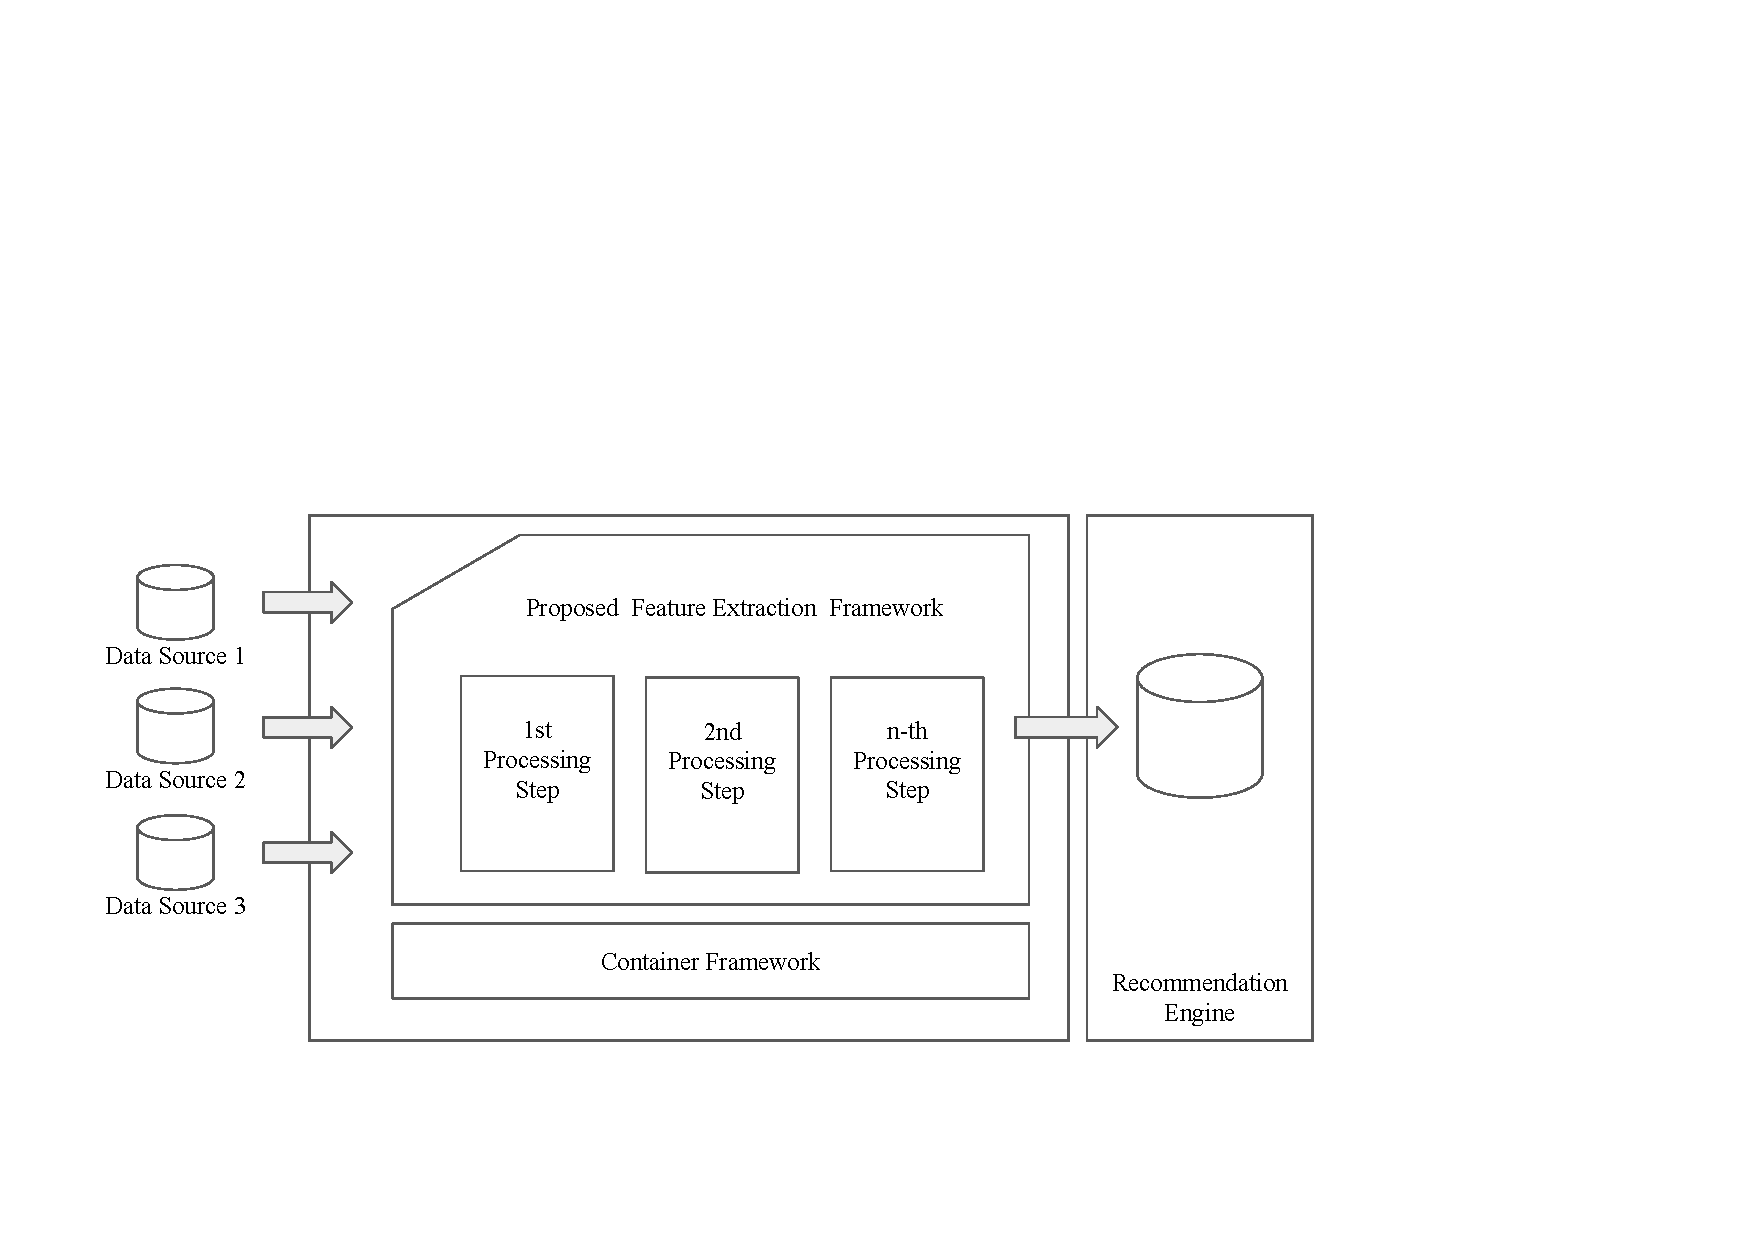
\includegraphics[width=0.9\textwidth]{framework-sketch}\\
  \caption{Feature extraction framework}\label{fig:framework-sketch}
\end{figure}

\section{Outline\label{sec:outline}}

In this section we well have a short overview of the chapters in this thesis. This work is separated into 7 chapters.
\\\\
\textbf{Chapter \ref{cha:chapter2}} covers aspects about fundamentals and related work. As state above the thesis follows a problem driven approach, therefor the underlying structure and problems of modern data storage concepts are analyzed, broken down in subproblems and finally assessed.
\\\\
\textbf{Chapter \ref{cha:chapter3}} uses the findings of chapter \ref{cha:chapter2} and develops requirements on the proposed framework. An additional explanation of each individual requirement is given to demonstrate its necessity.
\\\\
\textbf{Chapter \ref{cha:chapter4}} uses the specifications and requirements from chapter \ref{cha:chapter3} and elaborates in a top down approach a concept for an automated framework for feature extraction. Different aspects regarding the problems of chapter \ref{cha:chapter2} are covered and abstract solutions and concepts are introduced. The overall concept aims for a subsequent reference implementation of the suggested framework.
\\\\
\textbf{Chapter \ref{cha:chapter5}} describes the implementation of the suggested framework. A research on underlying technologies, the choice of a implementation language as well as structural decisions are conducted. Components on different layers are explained and applied patterns discussed. 
\\\\
\textbf{Chapter \ref{cha:chapter6}} interprets the findings and outcomes of the precedent three chapters. The discussion of the applicability of the proposed framework is lead under the aspect of the reference implementation. The concepts are challenged and cross-checked for their feasibility under a technical perspective.
\\\\
\textbf{Chapter \ref{cha:chapter7}} summarizes the thesis, describes the problems that occurred and gives an outlook about future work.
    \chapter{Fundamentals and Related Work\label{cha:chapter2}}

\section{Fundamentals in data unification\label{sec:unification}}

Electronic data processing underlies applied math and relies therefor on data of a certain, deterministic structure. In mathematics and computer science such rules of data representation are called canonical or normal form. Canonicalization is the discipline of transforming data of possible different forms of representation into a standardized form. An illustrative example of canonicalization is the representation of a boolean variable described in the XML schema type definition. By definition a boolean variable supports binary logic representation, meaning that some state or flag can either be true or false. The set of possible literals might contain: 1, 0, true and false. The XML schema type definition defines the canonical form of boolean as true and false, whereas 1 can be mapped to true and respectively 0 to false. Data in a normalized form can be transfered in any other form.
\\\\
The foundation of the idea of storing large data in a reusable format were captured by Edgar F. Codd in 1970 with his proposal for database normalization. The concept behind the proposal is to break the information down into entities with attributes and describe relations among them. A second and third version of database normalization followed and proposed a higher granularity. The technique of data normalization is state of the art in rational database systems. Such a system stores data in a table format, where rows correspond to entities and columns to their attributes. Considering the entities person and address as an example. The person entity has the attributes surname and name, the address entity the attributes street, zip code and city. In addition the person entity has a reference to the address entity, thus a an address can be related to a person. This relation is realized by a unique key. The system enforces the entity definition, i.e. its schema and the predefined data types, and the relationship constraints strictly. Relationship modeling plays also a fundamental role in other data base and data management systems but are often not enforced on system level.
\\\\
% https://db-engines.com/en/blog_post/23
In contrast to relational databases, normalization is not mandatory in non rational, also call no SQL databases. This kind of databases are mostly used for web applications and in the field of big data. The same applies to entity relationships as the core concept of no SQL databases aims for de-normalized data storage. Considering the person-address example from above, all attributes of a person entity are stored with it, including its address. No SQL databases exist with a schema-leas approach, meaning there is no predefinition of attributes and corresponding data types. This also enables changes of the schema over time in the cardinality of attributes as well as their type. In the person-address example this means that the address is a non mandatory field and the zip code can be stored as number or string. Document-orientated databases, key-value storages and graph databases are the three most common no SQL databases.  Limitations are only set by the user's definition and imagination. This flexibility enormously supports the initially claimed chaotic data storage, though it is often limited by schema definitions on domain level. 
\\\\
Schemas help to maintain a understandable structure of data and underly a certain format. They add determinism to data and make them less error prone. Schemas vary in their strictness, also formats allow different levels of precision. CSV, JSON and XML are the most commonly used formats for data interchange, whereas JSON holds a distinguished position nowadays. From a top down view on entity level they define the set of attributes an information entity has. In addition it is possible to define whether a field is mandatory or not. Furthermore a schema can be designed such that it enforces entity relations. On attribute level the most common specification is the data type, whereas the information if a field can be unset, i.e. nullable, can be provided too. Data types are usually not unique through different schema formats, but mappings usually exist. For a higher quality of data the individual type of an attribute can be restricted through ranges or enumerations, e.g. the value of field score can only accept integers from 1 to 5. Furthermore it is to distinguish between externally defined and self-contained schemas. External definition or external enforcement is the approach that drives rational databases and schema-full data storages. Is the schema woven with the actual data, one can speak about self-contained schemas. Schema-less storages benefit from self-contained schemas. Using such, data integrity it is for the application level to maintain.
\\\\
The canonical form standardizes data representation, whereas normalization and schema definition add some additional information to it. A predefined cardinality of attributes as well as the respective types and value ranges can be considered as meta-data and make the data therefor more understandable by human as well as by machines. 

\section{Data storage technologies and data formats\label{sec:storage}}

In data driven applications the data are commonly fetched from a source. Sources in this circumstances are wide-ranging. A few to mention here are:
\begin{itemize}
  \item Purely file based, e.g. CSV files
  \item Database systems (rational database management systems, key-value stores, document-orientated)
  \item REST interfaces
  \item Web sockets
  \item Message queues\\
\end{itemize}

\noindent\textbf{Purely file based} have almost no restrictions regarding the information format. The format is often defined on domain level. Human readable formats like CSV, JSON, XML or custom formats are some of the most common data structures. Additionally binary formats exists but are more often used in closed systems.
\\\\
\textbf{Database systems} provide more boundaries when it comes to the data format. Database management system can be divided in schema-orientated and schema-less systems. The former, by definition, enforces a certain schema for individual information entities. In rational database systems most often a table format is chosen, but also in key-value stores the format of the value might be enforced by the system. Schema-less systems, also often document-orientated, bring more flexibility. The format, in many cases JSON, has to be defined per type of information entities. The actual schema, i.e. definition of attributes, is not enforced in such systems.
\\\\
\textbf{REST interfaces} deliver data in most cases in human readable format. Some exception exist that expose binary information. The so called media type, also MIME type or content type, is officially standardized by the Internet Assigned Numbers Authority (IANA). Dedicated content delivery APIs mostly utilize pain text, JSON or XML. For memory reduction zipped data are shipped. 
\\\\
\textbf{Web sockets} are originally designed for the communication between browsers and web servers and lower network layer, TCP, as REST interfaces for data exchange. Projects exists where web sockets are used for data transfer and enables a streaming unlike REST, which works on a batch basis. Regarding data formats, web sockets apply similarly loose restrictions regarding formats as file based data sources does.
\\\\
\textbf{Message queues} are old techniques but embrace over the last years enormously. The trends shifts towards data streaming and directly process them rather to store data over the long-term. Often used for connecting systems, message queues do most often not enforce a specific data formats also similar to file based sources.

\section{State analysis of heterogeneous data storage\label{sec:stateanalysis}}

\begin{figure}[htb]
  \centering
  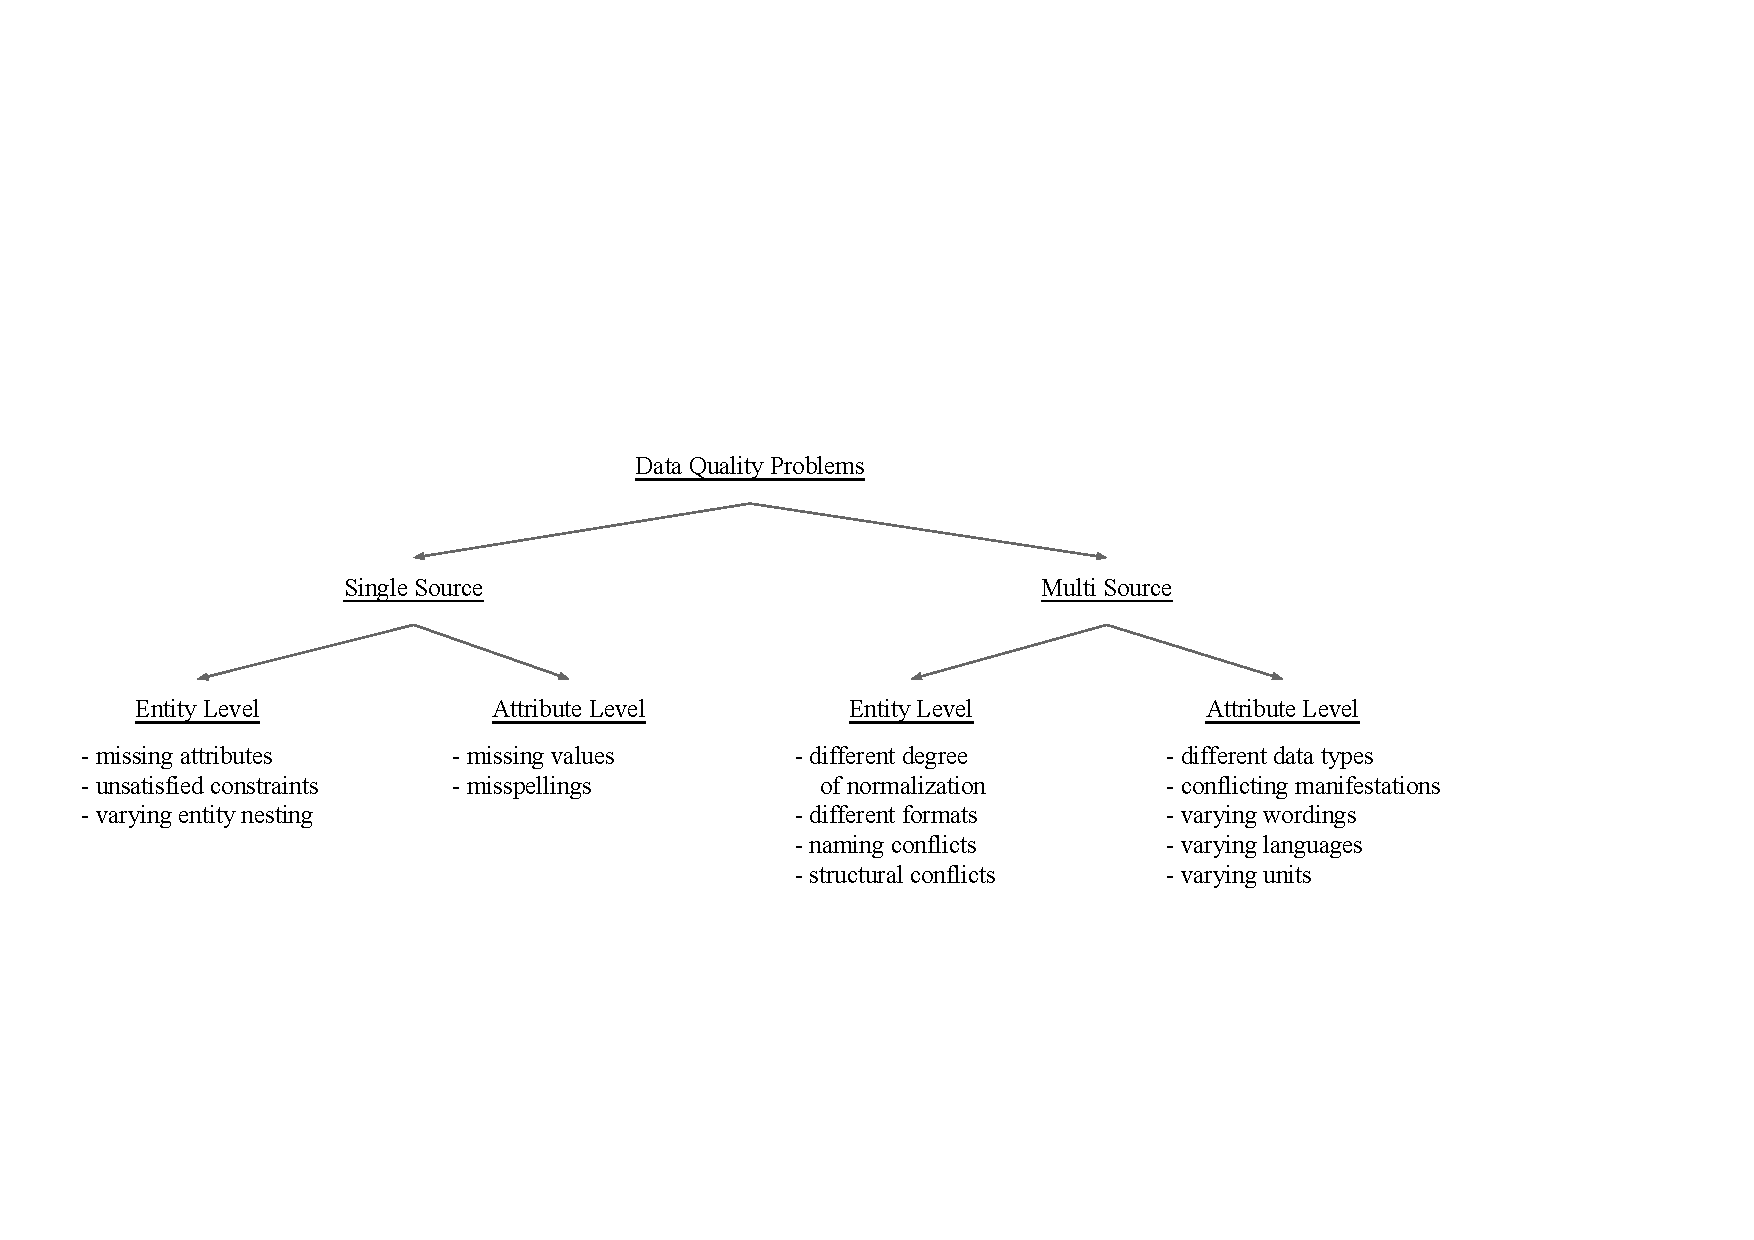
\includegraphics[width=0.9\textwidth]{quality-problems.pdf}\\
  \caption{Categorization of data quality problems}\label{fig:qualityproblems}
\end{figure}

In this section digitally available data are analyzed with respect to their quality as well as considering their source. Figure \ref{fig:qualityproblems} illustrates a categorization of the data quality issues into four sub problems. The breakdown shows that the devision correlates with the above stated classification of data storage principles. Therefor a general distinction between single and multi source problems is possible. In both categories a distinction on entity level can be made. 

\subsection{Single source problems}

Single source problems consider malformed data within one storage system. A single source normally is maintained by a single instance and can be considered as less messy as a multi source environment. Nevertheless even such system contain malformed data which can not be directly used for analysis.

Schema-less systems can be considered as more error prone than systems enforcing a schema. In the former unsatisfied constraints occur whereas in the latter additionally missing attributes and varying entity nesting arise. Those problems are mostly schema related and occur due to poorly designed schemas, technical depts or negligence of specifications. Attribute level specific issues can only partly covered by schema definitions. For instance, missing values are coverable but not spelling errors. Table \ref{tab:singlesource} outlines examples conflicts occurring on data unification. 

Missing attributes or missing values no not necessarily indicate malformed data. Information entities exist where the absence of data actually provides insights. Declaration on specification level increases the interpretability and analyzability of latent information accordingly. Broken constrains reflect inconsistent and missing data. Compare row one of table \ref{tab:singlesource}.

The second row of table \ref{tab:singlesource} shows an person entity referring to a non-existing address. Data are not usable under original condition and has to be re-interpreted. In document-orientated databases can be nested within sub-entities but basically providing equal information. On unification such data structures conflict and require exceptional treatment. 

% TODO nesting

Another potential conflict arises when it comes to standardizing data are missing values. An example is provided in row four of table \ref{tab:singlesource}. Unset values can be interpreted in two fashions. It can mean on one hand, that the value for that attribute is not captured, i.e. the value exists but is not present, on the other hand it can imply that it can not be captured, i.e. the attribute is not available for that entity. Whereas the former is the correct interpretation in terms of data management, it is widely abused in the sens of the latter definition. The interpretation is up to the maintainer of the data source. A further problem in both cases are missing values on mandatory fields in respect of future data processing.

Misspelling are faulty data from manual entry. The problem of such when it comes to heterogeneous data aggregation is the same problematic as in homogeneous environment and therefor plays a very critical role for example if information are displayed to end users.  

\begin{table}[htb]
\centering
\resizebox{\textwidth}{!}{
\begin{tabular}[t]{|l|l|}
\hline
Problem & Example \\
\hline
\hline
Missing & Person\textsubscript{1}(name="Fritz", age="23", city="Berlin") \\
attribute & Person\textsubscript{2}(name="Eva", city="Berlin") \\
\hline
Unsatisfied & Person\textsubscript{1}(name="John", addressId="1") \\
constraints & \\
\hline
Varying entity & Person\textsubscript{1}(name="Fritz", street="Spanische Straße 17", city="Berlin") \\
nesting & Person\textsubscript{2}(name"Eva", address=Adress(street="Baumallee 34", city="Berlin")) \\
\hline
Missing & Person\textsubscript{1}(name="Fritz", age="23", city="Berlin") \\
values & Person\textsubscript{2}(name="Eva", age="", city="Berlin") \\
\hline
\end{tabular}
}
\caption{Examples of single source problems}
\label{tab:singlesource}
\end{table}

\subsection{Multi source problems}
All problems from a single source environment can be transfered to a multi source environment. Additionally the absence of commonly valid schema definitions fosters problems when it comes to unification of data and information among various sources. The sub categorization of multi source problems goes along with the sub categorization of single source problems. On entity level issues due to different degrees of normalization, different formats, naming conflicts or structural conflicts are possible discrepancies. On attribute level different data types, conflicting manifestations, languages and units prevent a simple solution to data unification.

One big challenge in data source fusion is a different degree of normalization or granularity of data. Highly depending on the use case the data are collected for, attributes are broken down into different abstraction levels. For that reason one attribute in one source can correspond to two or more attributes in a second source. Depending on the storage technology used the same information are de-normalize, i.e. one entity captures all information, or completely normalized, i.e. split up into two entities. Row one in Table \ref{tab:multisource} shows three information entities that basically contain the same data but in different forms of normalization. Normalization of fields requires in some cases significant domain knowledge. 

Section \ref{sec:unification} provided an overview of different data formats. Every one has its on semantic and characteristics. A straight forward aggregation among two data formats is barely possible. For instance, comparing the JSON format with CSV shows, the first supports nesting of entities the other not. XML and JSON on the other hand support both nesting but distinguish in incompatible data types, as JONS for instance can not represent long integers, whereas XML supports this data type.

A well known problem is the parsing of addresses, especially street names and house numbers. From an automation point of view it is impossible to perform accurate splitting of that fields. This is a crucial point if the desired output format requires a higher degree of normalization than some of the underlying sources can provide. Row two in table \ref{tab:multisource} shows an example of different schema definition in terms of attribute naming. Fields containing equal information are annotated by a different name. In this example the fields \textit{city} and \textit{town} contain the home town of the person captured. This heterogeneity can also be the source of usage of different languages, e.g. American English and British English. 

As already explained in \ref{sec:unification} storage formats support different data types. Not only technical restrictions but also domain specific restrictions require a different choice of data type for the same type of information. As an example we can consider the ZIP code. For some countries it is sufficient to use an integer type for others its is mandatory to store the postal code as string, as non-numeric characters are contained. Compare row three in table \ref{tab:multisource}. 

Enums provide a predefined set of manifestations for a certain attribute. Usually designed to avoid messy data enums can in fact cause discrepancies during data unification. This problem is similar to the attribute naming problem mentioned above: Different manifestations stand for the same information value. The problem becomes more severe if a direct mapping among sources into one distinct target format is not possible. In system A a entity can accept n different states, whereas in system B m different states are possible. See row four in table \ref{tab:multisource} for comparison.

Similar to differing manifestations is the problem of different units. Two example entities can be seen in row 5 of table \ref{tab:multisource}. The problem is of a higher complexity as quantities are also affected. Especially for mathematical data analysis a common system of units is essential. Combining data from multiple sources must consider such inequalities otherwise aggregations results are faulty.

All multi source problems can be applied as outlined here to schema-less data storages. 

\begin{table}[htb]
\centering
\resizebox{\textwidth}{!}{
\begin{tabular}[t]{|l|l|}
\hline
Problem & Example \\
\hline
\hline
Different degree & Person\textsubscript{1}(name="Fritz", address="Spanische Straße 17, Berlin") \\
of normalization & Person\textsubscript{2}(name="Eva", street="Baumstr.", no="34", city="Berlin") \\
 & Person\textsubscript{3}(name="John", adrId="1"), \\
 & Address(adrId="1", street="Weg", no="2", city="Berlin") \\
\hline
Naming & Person\textsubscript{1}(name="Fritz", city="Berlin") \\
conflict & Person\textsubscript{2}(name="Eva", town="Berlin") \\
\hline
Different & Address\textsubscript{1}(zip="24821", city="Berlin") \\
data types & Address\textsubscript{2}(zip=24821, city="Berlin") \\
\hline
Different & Product\textsubscript{1}(name="apple", status="new") \\
Manifestations & Product\textsubscript{2}(name="apple", status="created") \\
\hline
Different & Product\textsubscript{1}(name="apple", amount="1", unit="ea") \\
Units & Product\textsubscript{2}(name="apple", amount="1", unit="kg") \\
\hline
\end{tabular}
}
\caption{Examples of multi source problems}
\label{tab:multisource}
\end{table}

\section{Assessment of problems for feature extraction\label{sec:problemassesment}}

Based on the previous section an assessment of the revealed problems. Indicator as their severity and complexity are considered and finally used to identify concrete issues handed within this work. 
\\\\
Unsatisfied constraints are a general problem in no SQL systems and need to be enforced on application level. Broken constraints are therefor not considered as a major problem of homogenization of data sources. The same applies to misspelling errors. This type of error is required to run through spell checking software and needs extended manual quality checks for appropriate correction. 
\\\\
The main focus in this work will be on unifying data for automated feature extraction that underly the problems of structural issues. Automation technologies an methods need to be identified and applied reasonable. This covers the sub problem like missing attributes, naming issues and varying entity nesting.
\\\\
As second aspect differing levels of normalization are in the focus of this thesis. This is due to the fact, that preliminary information from modern storage systems, e.g. schema-less databases are to be analyzed as they make up a significant amount of latest data in web applications.
\\\\
As third an last main focus problems towards different manifestations are chosen. Especially categories and labels for data are very important in modern machine learning approaches. Features extracted from this kind of information provide value in applications like predictions and recommendations.

\section{Available Technologies \label{sec:tech}}

This section describes relevant technologies, starting with X followed by Y, concluding with Z.

* ETL

    \chapter{Requirements\label{cha:chapter3}}

After defining the main problems and objectives to be handled in this work in the previous chapter, this chapter defines the requirements for an automated system that extracts well defined characteristics from heterogeneous data. The requirements are engineered from a top down view.

\section{Overview\label{sec:reqoverview}}

The primary goal of this work is to design an automated system. Any type of automated system require a interaction point for quality check and quality assurance. Furthermore it is required by the system to evolve over time such that the performance maximizes and manual interactions can be minimizes. This also plays a role when it comes to adapt additional data sources. The maintenance effort on such an interference must kept at a minimum, as well as on development side and quality assurance side. The framework should be designed as such, that a continuous processing of semi-structured data is possible at all time. Hence, it must be fault tolerance towards unexpected input and also provide a interaction point to assure processing of faulty data.
\\\\
The following points summarize the requirements for the proposed framework:
\begin{itemize}
\item High degree of automation
\item Self learning system
\item Easy adaptability of data sources
\item Error resistant and processing guarantees
\item Schematizing data output 
\end{itemize}

\section{High degree of automation}

A system meeting the demands of high degree of automation defines it self as a system that delivers data on a continuous bases with stable quality and minimal manual interactions. Here we can distinguish between manual interactions on data preparation and quality check. Especially on sensitive data manual overhead for quality assurance can not be prevented. Nevertheless the finalizing operation must kept at a minimum. Hence the requirement here is a interaction point that ensures the latter demand. The second requirement in this paragraph is continuous pre-processing of newly incoming data.

\section{Easy adaptability of data sources}

As already stated in chapter \ref{cha:chapter1} the amount of data is rapidly growing every day. This also implies of newly emerging data sources on a high frequent basis. This fact leads to one requirement of a system that automatically extracts information characteristics is the adaptability to additional data sources. This requirement ensures the gathering of a wide range of data leading to a versatile data basis, which is indispensable for applications like content delivery platforms and recommendation engines.

\section{Self learning system}

Continuous delivery of high quality data features can only be realized if the system adapts to trends and learns from feedback of quality assurance. This is a very natural way of increasing performance. Capturing all possible manifestations of data i.e. wordings, semantics or ontologies, at specification phase is not desirable and truly not possible. Hence, it is required for the system to extend its definitions and widen the underlying knowledge base. 

\section{Error resistant and processing guarantees \label{sec:error}}

This requirement aims for fault tolerance on domain level. As already outlined, discarding faulty data will result in faulty results. Compare paragraph 'Mathematical analysis' in section \ref{sec:moti}. But on the other hand, implementing a system that can process 100\% of messy information to well defined data is an unreachable goal. Unexpected and faulty information entities occur in every system on a regular basis. Due to that, the Framework must be designed such that processable data are not ignored nor discarded. The requirement is to define a technique that guarantees the capturing of all information entities.

\section{Schematizing data output}

For professional data analysis it is essential that the resulting data comply with and generalized, predefined schema. As explained in section \ref{sec:unification} globally valid and well defined schemas on top of of standardized data is the requirement for data processing, visualization and analysis. For different data applications different schemas are necessary. Therefor the last requirement of the proposed framework is a convenient mechanism to exchange or extend the output formats. 








    \chapter{Concept\label{cha:chapter4}}

Not only the requirements form the previous chapter \ref{cha:chapter3} but also the analysis and assessment of faulty data in \ref{cha:chapter2} is the basis for concept design of the resulting framework proposal. This chapter introduces the design of the overall framework and its components as well as its architectural design.

\section{Overall framework design \label{sec:overalldesign}}

\begin{figure}[htb]
  \centering
  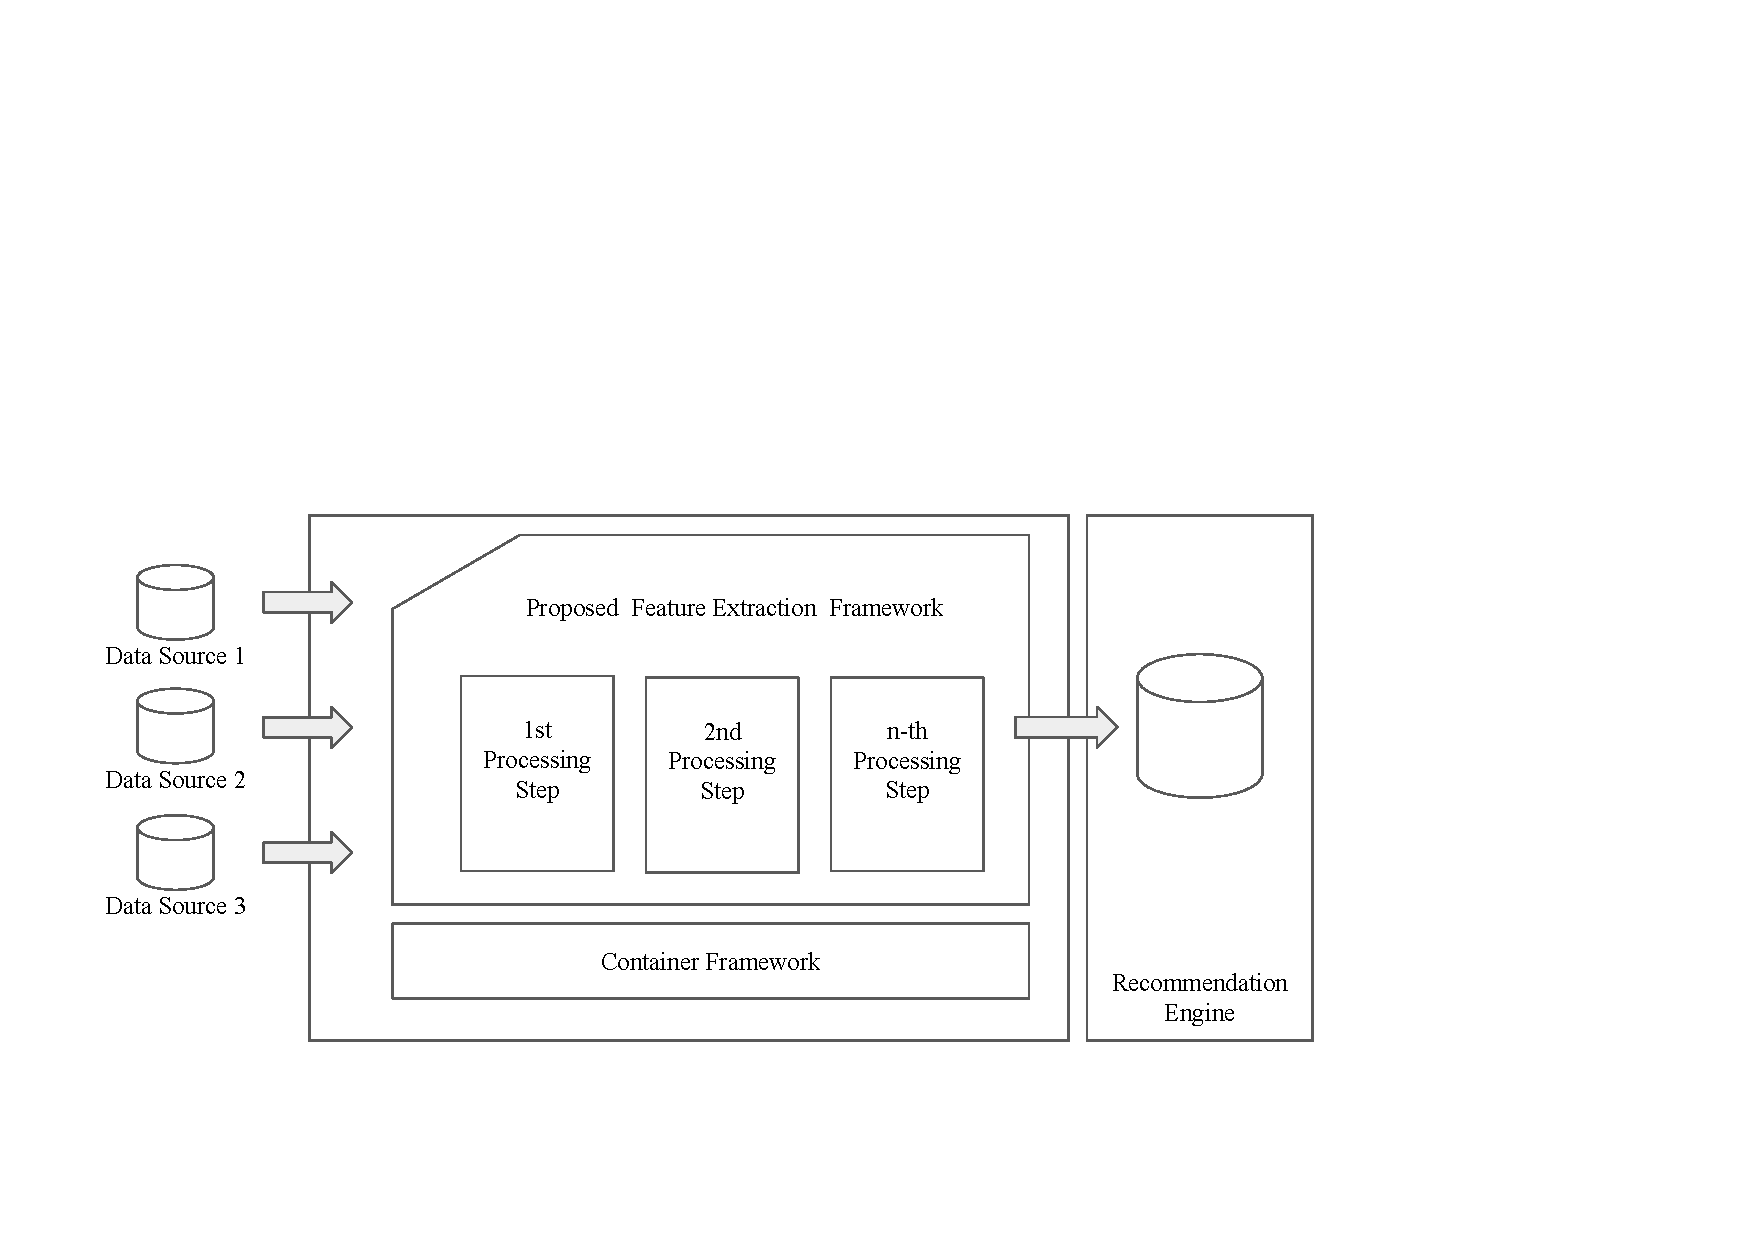
\includegraphics[width=0.9\textwidth]{concept-framework}\\
  \caption{Basic concept of feature extraction framework}
  \label{fig:basicconcept}
\end{figure}

To satisfy the requirements of simple adaptability and reliable system a modularized framework concept is applied. A pipelined approach with adaptable components characterizes the overall framework design. A software application of the proposed framework is desirable. Therefore, modularized software design and development ensures a level of abstraction that aims for simple update, exchange or addition of features. Single modules are implemented encapsulated and exchange data via APIs on different transportation technologies. Common data structures and interfaces are shared via libraries which are simply a further module of the framework. Namely \textit{core} or \textit{common} libraries in various software projects. Compare modules and components, also available as libraries, of the Apache Fink framework. % https://mvnrepository.com/artifact/org.apache.flink
\\\\
Revisiting the in chapter \ref{cha:chapter3} stated requirements leads to the breakdown of the framework into the following modules:
\begin{itemize}
\item Source adapters
\item Parsing pipeline
\item Output adapter
\item Error pipeline
\end{itemize}
In addition to handle underlying data transfer and processing a container framework is used. This simplifies the implementation of the feature extraction framework and abstracts the heavy lifting of data processing.
\\\\
The pipeline concept facilitates the handling of single and multiple source problems analyzed in chapter \ref{cha:chapter2}. A three step approach towards clean features is chosen to tackle structural problems and issues on entity level at once. Internally the framework must use a one data schema to reduce overhead on transformation as well as introduction of errors.

\section{Concept and use of the container framework \label{sec:containerframework}}

Many data processing frameworks are available nowadays. Especially the trend of big data emerged frameworks on different abstraction layers. Most of them have their foundations in widely known concept of Map Reduce or any of its descendants. Promising Open source examples in this case are among others Apache Flink, Apache Samza, Apace Spark or Kafak Streams. Conceptual the container framework hides away underlying data transportation and enables the use of user defined code and user defined functions. There the in the previous paragraph mentioned modules can introduced. This abstract concept will allow to exchange the underlying container framework as well as consecutive modules. In the next chapter, chapter \ref{cha:chapter5}, after evaluation of different container frameworks the best suitable is determined.

\section{Concept of the input adapter \label{sec:inputadapter}}

The input adapters are mainly responsible for format and schema specific generalization of incoming data. The drawbacks of heterogeneous file formats is covered in section \ref{sec:stateanalysis}. From this we know it is essential to find a common and flexible way to represent data within one system. The concepts does not make any suggestions regarding the format to be chosen, as the framework must not rely on implementation specifications. It only suggests that one common schema for the entire framework to avoid translation overhead and internal error sources. For a generalization purpose the concept defines a library which enables an easy adaption to multiple data sources, their formats and schemas. The formats can be found on the y-axis in figure \ref{fig:inputadapter}. As we speak about data unification in this work, on the other axis the raw entity type can be found. For instance, if the features for animal entities have to be found across different sources the library provides a tool set to define as the input format and the output schema. Furthermore the input adapter provides the functionality to combine a specific input source with a specific output entity an an abstract level. In a concrete case the developer must have a interface provided to define the source depended schema and a user defined function (UDF)\footnote{A UDF is a function that is executed in a bigger context, accepts parameters performs non-side-effecting transformation and returns the result} to map between source schema and the raw target schema. Additional source depended knowledge can be applied on the data. For instance, internal quantities and units can be transformed to international standards. The concept defines a library which plugs in a custom source schema on a predefined (or custom) data source, mapping function to translate the source schema and the definition of the raw target schema. The UDF has a very simple interface, as it is defined as a function mapping a source custom source schema to a raw target schema. The raw schema does not support deterministic values but defines a set of attributes necessary for further processing steps.

\begin{figure}[htb]
  \centering
  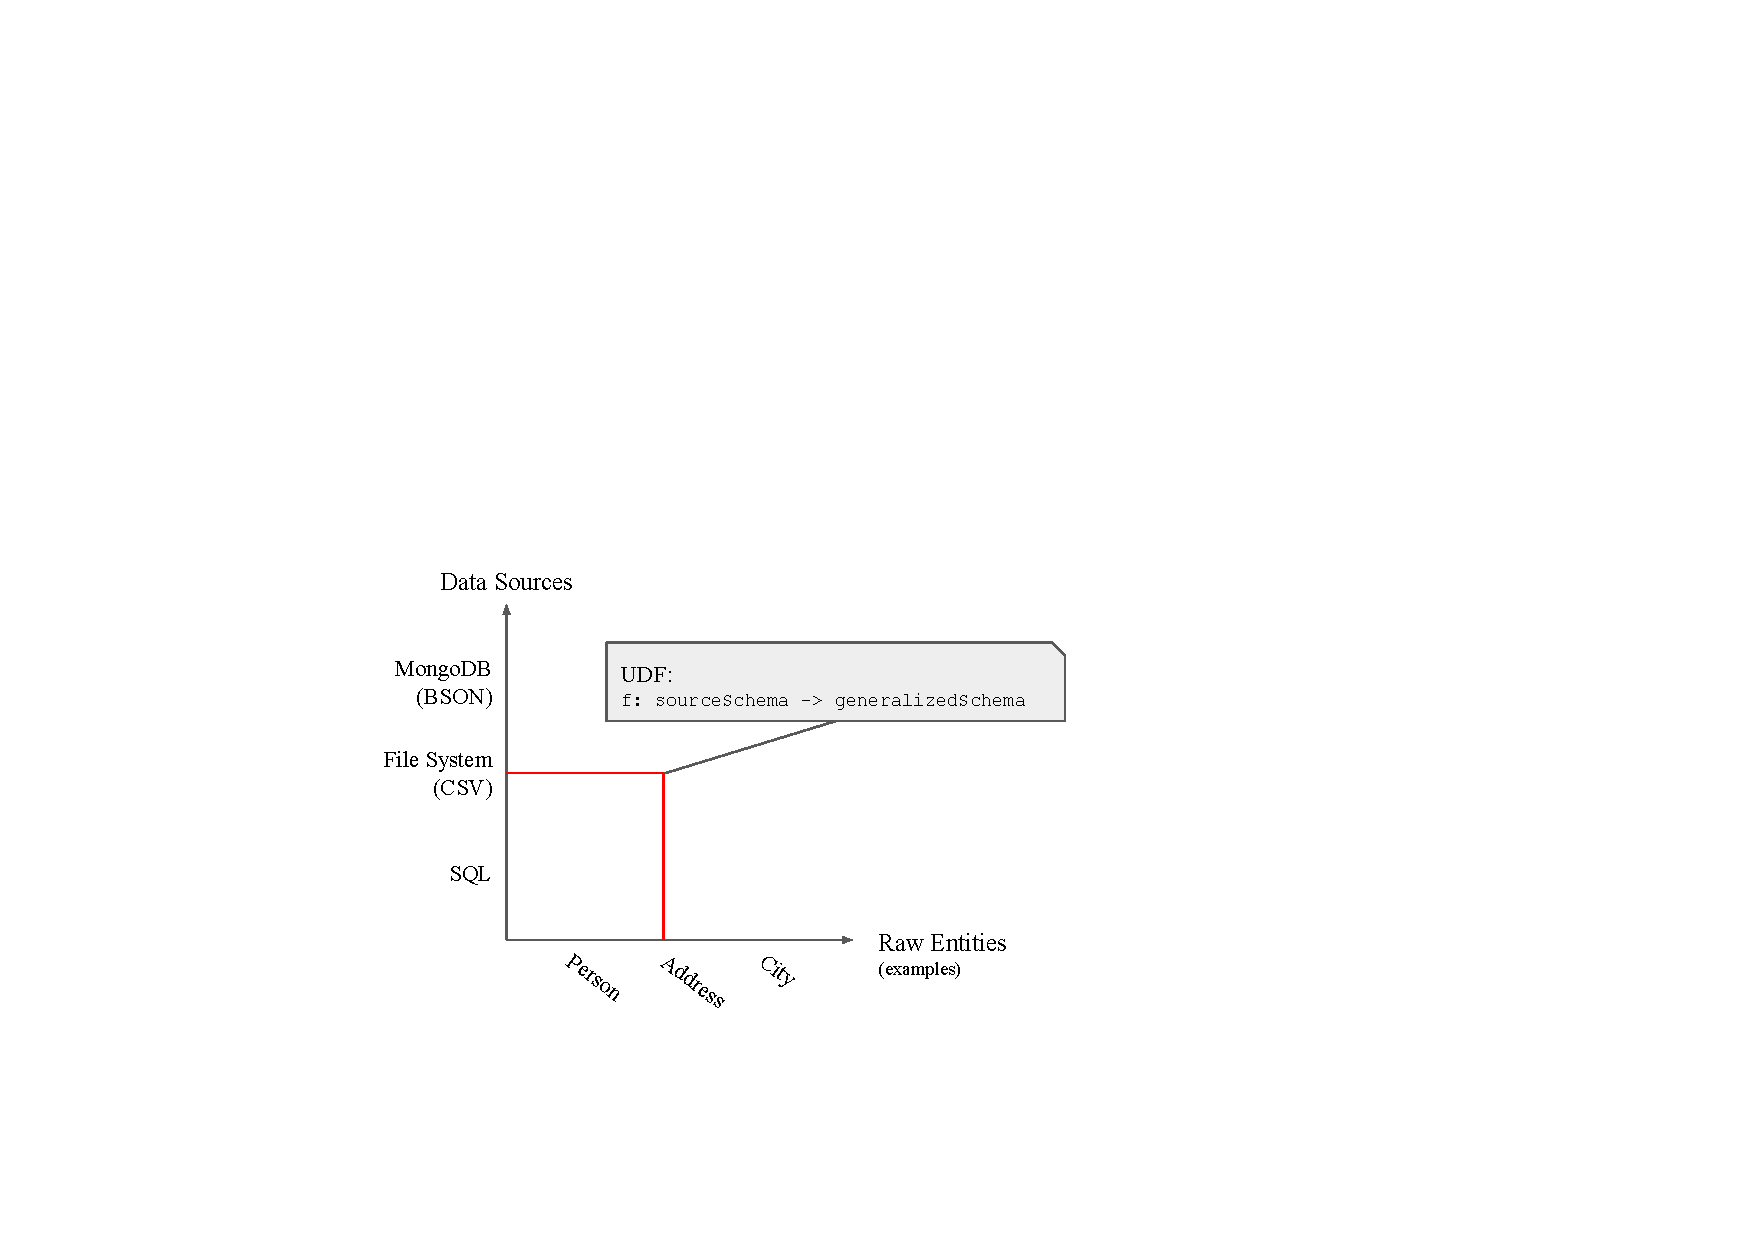
\includegraphics[width=0.6\textwidth]{input-adapter}\\
  \caption{Concept of input adapter library}
  \label{fig:inputadapter}
\end{figure}

\section{Concept of parsing pipeline}

The core of the processing framework is the centralized parsing pipeline. At this point the raw schema is transfered to a generalized schema. The difference here is that the raw schema can be considered as stable and therefore adequate transformation can be applied. The concept suggests that the transformation is split up in different steps which perform different types of computations on the respective raw entity. The generalized schema is to be provided by a developer but is committed on domain level in which the proposed framework is operating. As already explained in the previous section, section \ref{sec:inputadapter}, the concept of UDFs provides a flexible method of introducing custom functionality into a predefined system. For the parsing pipeline the same approach is applicable, as the raw entity is transformed over a deterministic number of steps towards a generalized schema. 
\\\\
Possible parsing steps among others are:
\begin{itemize}
\item Unification of different levels of normalization
\item Source independent transformation
\item Homogenization of attribute value manifestations
\end{itemize}

The abstraction of an parsing step must allow the connection to a second data source for potential data enrichment through lookups. Another obligatory feature is a initial loading of a user defined resource such as a mapping table or a model. For this type of application of the processing pipeline a asynchronous processing should be possible to avoid a blocking of the pipeline.

\section{Concept of pluggable output adapters\label{sec:componentsoutput}}

The pluggable output adapters are meant for further transformations of the generalized entity that results from the parsing pipeline. Based of different intents of using the homogenized data, a set of outputs is desired. This boils down to data formats that are required by the acutaly application downstream of the feature extraction framework. From a framework aspect the output adapter is similar to the input adapters. The concept differs in a deterministic input as well as output schema or a set of deterministic schemas, depending on the post-processing use cases. The input schema is analog to the final output schema of the parsing pipeline and due to the fact of a unified format within the overall framework does not produce additional development overhead. 

\section{Concept of error pipeline \label{sec:errorpipeline}}

From the requirements (chapter \ref{cha:chapter3}, section \ref{sec:error}) a concept for error persistence and processing guarantees is developed. The overview in figure \ref{fig:basicconcept} show a component called \textit{Error Pipeline}. The idea of the error pipeline is to create a bypass stream of faulty data. Faulty data are defined by the fact that they could not processed in any steps of the framework. Faulty data from different steps of processing must be marked with the kind of error and the step where the error occurred. This must be done manly for a administrative purpose and manual quality check. Therefor the data can be located in different streams or data collections from where they can be fetched to analyze the underlying problem.

\section{Concept of quality assurance and ability of administration}

The quality assurance component of the automated framework is and overreaching element. Already lined out in section \ref{sec:errorpipeline}, occurring errors need to be handled. Other tasks to perform from an quality aspect are the control of the ongoing learn process of the entire system. Configuration of parsing rules and updating of mapping references are features to be controlled through an admin interface. For that, the system needs to be defined such that on different entry points over the modules interactions can take place. This is special for the parsing pipeline. As already explained, singular steps are configurable from the outside. The concept defines a dedicated interference point such as a database or data storage. Furthermore the injection of of quality concerns right after parsing but before sending data downstream through the output adapters is implemented. Manual crosschecks through an interface are enable. Additionally the manual introduction of generalized data satisfies the need for the required processing guarantees. 
    \chapter{Reference implementation of suggested framework\label{cha:chapter5}}

This chapter describes the concrete implementation of common aspects of the proposed framework as well as individual domain specific implementation. The in the concept, compare chapter \ref{cha:chapter4}, described introduction of libraries to enable an simple and adaptable solution is applied on the common aspects of the framework. The domain specific implementations provide an evidence about the generalization of the common elements as well as the applicability of the entire framework to specific domain. This chapter also discusses technologies as basis of the framework. 

\section{Environment and underlying frameworks\label{sec:env}}

\subsection{Technical container framework}

The use of the technical container framework promises the abstraction and simplification data processing frameworks offer. Using such a framework contributes a stable environment as basis. Under the consideration of the outlined concept, especially the pipeline approach, the best fitting container framework is chosen from the family of stream processing frameworks. Stream processing enables a continuous delivery of prepared data, ships with features enabling processing guarantees.
\\\\
Consequently the following alternatives must be considered as container framework:
\begin{itemize}
\item Native stream processing engine of high level programming language
\item Distributed stream and data processing frameworks
\item Single node 3rd party stream processing frameworks\\
\end{itemize}

\noindent\textbf{Native stream processing engine of high level programming language:}

\noindent High level programming languages like Java already provide a library for processing data as a stream\cite{urma_2017}. The offer the basic data processing functions like \textit{map(.)}, \textit{fold(.)} or \textit{filter(.)}. The barrier of applying a native stream processing framework is compared to external libraries relatively low as the nature of the language is preserved. Another benefit from using such a library are lower compatibility issues and fewer external dependencies. It is to favor to reduce maintenance overhead of software by reducing the number of external dependencies. 

The main drawback of internal processing engines is often that the connectivity to data sources and data sinks is limited. For example do Java streams only provide a connector to files in a local file system. If databases or message queues are plugged in custom stream sources need to be implemented. As the overall goal of the proposed framework is the unification of data across several sources native stream processing engines can not be considered in this concrete implementation.
\\\\
\textbf{Distributed stream and data processing frameworks:}

\noindent In section \ref{sec:containerframework} we already spoke about the trend of distributed data processing frameworks. Framework like Apache Flink, or Kafak Streams are specialized on data processing and provide a solid environment of features required for the proposed framework. Especially the aspect of distributed processing seems interesting when it comes to big amounts of data. Such framework minimize the implementation overhead due to distributed memory management and network communication. They also provide a brought set of connectors to different data sources and sinks. For example Apache Flink lists 13 connectors to 3rd party sources\cite{flink_streaming_2017}. 

A minor drawback is the dependency on external developers. Every externally introduced program code can in the worst case contain bugs. Restrictions regarding features are set by other developers and their overall focus and road map of the library or framework. A more significant disadvantage is that this frameworks are designed to run on a distributed, clustered system. Some of the framework do in fact provide a local execution mode, but this is often only recommended for development purposes but not for production environment. Not only for the sake of simplicity also to minimize the the complexity of the system it is necessary to find a framework that allows single node deployment. It is also to mention, that throughput is not listed as a requirement for the feature extraction framework. It is also not to forget, that the frameworks concept is designed in such a ways, that it does not depend on the underlying data processing framework. Hence, if the requirement for distribution arises, the processing engine can be replaced.
\\\\

\textbf{Single node 3rd party stream processing frameworks:}

\noindent From the previous two paragraphs we learned, that a 3rd party stream processing engine is a desirable ways to go. The requirement for reducing implementation complexity of a showcase example brings the demand for single node deployment. Unfortunately the list of frameworks satisfying the restrictions above is short. The Akka framework for actors\footnote{A Actors model is a mathematical model enabling parallel and concurrent data processing.}\cite{akka_2017} enjoys a brought acceptance among developers. This framework provides a streaming framework on top of Akkas actor model. Akka streams\cite{akka_streams_2017} have a excellent support through the close relation to the Scala programming language as well as a wide community support\footnote{More than 400 contributors on https://github.com/akka/akka.}. Concerning the adaptivity of heterogeneous sources a community is established that provides connectors to more than 20 data sources, sinks, protocols and libraries. The Alpakka library\cite{alpakka_2016} contains among others connectors to the major database systems like MongoDB, Hbase or Cassandra, as well as to file formats as CSV, XML or text files. The repertoire of alpakka connectors also lists transfer protocols like FTP, which can be beneficial for integrating remote sources of customers on a file basis.
\\\\
For the proof of concept implementation of the automation framework Akka streams is chosen as the container framework and extended by the alpakka library. 

\subsection{Data transfer layer}
To maintain the concept of modularization and pluggable of the framework while using Akka streams it is essential to introduce a data transfer component. The data transfer layer is part of the assemble of technologies building the container framework. Singular components realized in Akka streams need to be connected through that data transfer layer. This component is also used for the realization of the error pipeline as described in section \ref{sec:errorpipeline}. An easy to use candidate for such an application is Kafka. The streaming platform works with a publish-subscriber pattern and is a fault tolerant system for connecting software components. The ability to create streams, known as topics, comes beneficial for the error pipeline. Here each step can define its own topic to which faulty data can be published and distinguished afterwards.

\subsection{Programming language and libraries}
The choice of the target programming language primarily depends on the application use case. Data processing and data transformation are often non-side-effecting applications of functions on single information entities. This can be seen on the concept of UDFs in the proposed framework. The conclusion can be made, that a functional programming language is well suited for this thesis' implementation. 

A second, very related aspect, is the API of the underlying framework. As the underlying framework is chosen by the best fit for the thesis' use case it is natural to imply that the technical container frameworks language is the right fit. 

Scala as a functional programming language combines the two previous aspects. This brings us to the conclusion, that the Scala programming language is a perfect candidate for a example implementation of the framework and development of the demonstrative use case.

\subsection{Internal data format}
The use of the data transfer layer urges the use of an internal common data encoding format. This aspect is already described in section \ref{sec:overalldesign}. Apache Kafka does not restrict the usage of certain data formats. Due the wide usage and human readability JSON is considered as a suitable internal data format. This also enables manual inspection of information entities on quality assurance tasks. 

\section{Implementation of input adapter and raw formats}

The implementation of the input adapter on the frameworks library level boils down to three main classes. A data loader, a data sink and a third component to wire up the former classes. 

\subsection{Implementation of the loader component \label{ssec:loadercomponent}}

A source specific data loader is a sub-class of the abstract generic class \textit{AbstractLoader}, compare the class diagram in figure \ref{fig:importer-diagram}, and is meant to hide the actual encoding format of the data source as well as to transform a source element of type \textit{IN} to raw type \textit{OUT}. A \textit{AbstractLoader} requires the implementation of the data source, which is defined as a \textit{Source}-object in the Akka streams framework and can be taken from the previously name Alpakka library. The abstract function \textit{tryParseElement($\cdot$)} is a function sub for the actual UDF that enables the mapping of the source schema of type \textit{IN} to the raw schema of type \textit{OUT}. The function \textit{handleFailed($\cdot$)} is called before an faulty element is written to the corresponding message queue in Kafka and can be overwritten in the case the user wants to introduce custom error handling.

As a concrete example a MongoDB loader was implemented and provided to to framework library. This example utilizes the ReactiveMongo driver\footnote{http://reactivemongo.org/} which is used to implement the Akka stream source as the class \textit{AbstractLoader} requires.

\begin{figure}[htb]
  \centering
  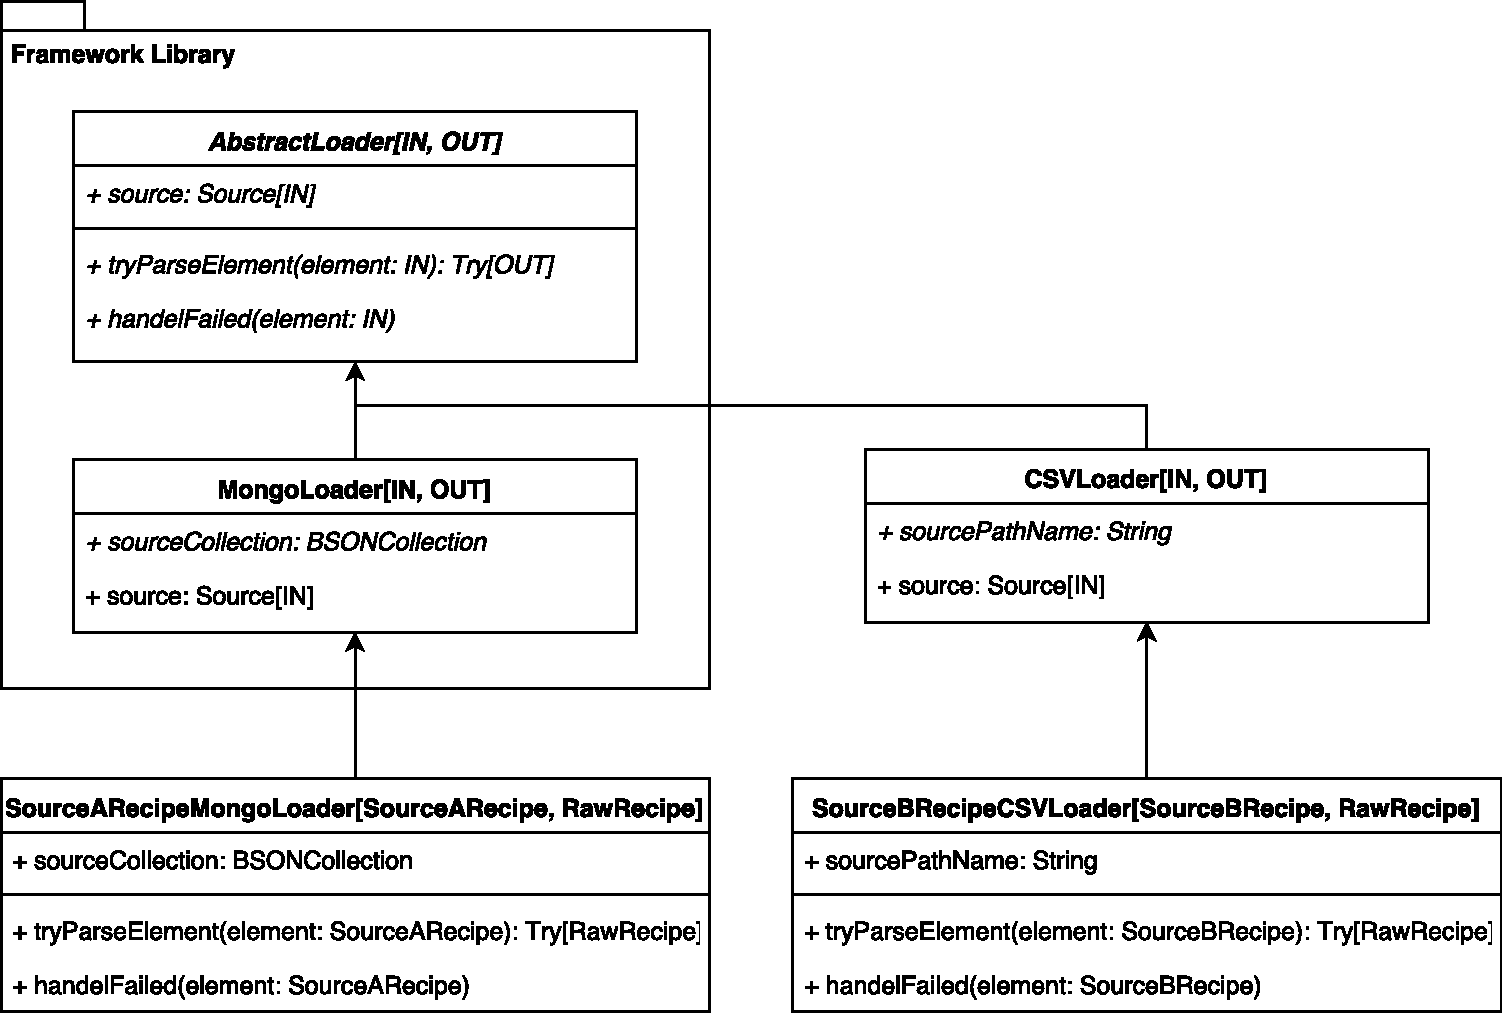
\includegraphics[width=0.9\textwidth]{importer-diagram}\\
  \caption{Class diagram of data loader library and implementation}
  \label{fig:importer-diagram}
\end{figure}

In the third level of the inheritance hierarchy the source and raw format needs to be specified. Here is also the implementation of the UDF located. The UDF takes a source specific element as parameter and must return a the defined raw entity. This is the only place where domain specific knowledge is introduced.

\subsection{Definition and introduction of raw entities}
In the framework a raw entity is defined as global valid abstraction of information entities among all possible sources. To satisfy this specification it is necessary to declare redundant attributes for different sources. Taking a recipe as example, investigation on available data shows that for example ingredients are normalized into three levels:
\begin{itemize}
\item "amount unit name"
\item "amount unit", "name"
\item "amount", "unit", "name"
\end{itemize}
To find one raw format that satisfies the most possible sources, three different attributes are introduced in the raw recipe entity. This approach enables downstream processing steps to apply adequate rules for each of the three attributes and extract the highest level of normalization \textit{"amount", "unit", "ingredient}. This level is desirable for post-processing applications that use features build on amounts of ingredients or their names. It is also thinkable to simply choose the lowest level of normalization if the downstream application does not need detailed information. From this example we see, that the introduction of the abstract raw entity satisfies messy source data as well as reliability for downstream preparation steps. It perfectly fits the idea of a modularized software.

This core approach is not only applicable for recipes and their ingredients. It can be simply be transfered to other domains like product catalogs or person profile information.

\subsection{Implementation of the sink component for raw entities}

\begin{figure}[htb]
  \centering
  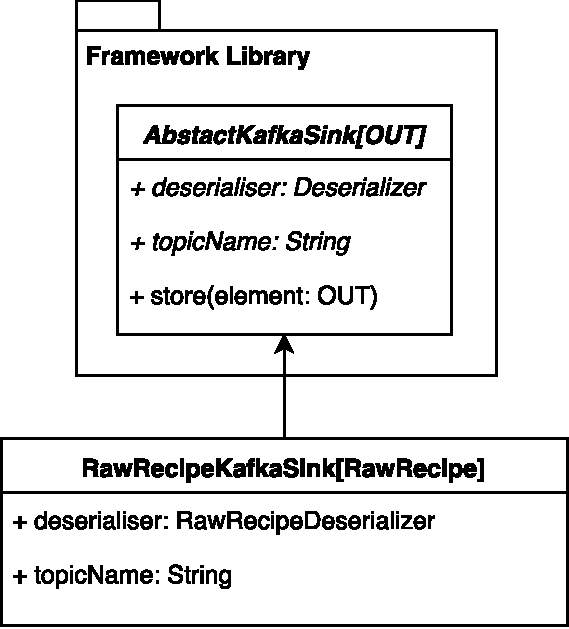
\includegraphics[width=0.3\textwidth]{importer-sink}\\
  \caption{Class diagram of input adapter sink and implementation}
  \label{fig:importer-sink}
\end{figure}

The second component from the input adapter is the sink to the underlying transportation layer. It is abstracted by the class \textit{AbstractKafkaSink}. The implementation must specify the serializer\footnote{A serializer is a software component, that defines how an specific class instance is created from a an different input format.} that is used to write the raw entity to the Kafka topic. Additional the topic name is to be provided. The class diagram in figure  \ref{fig:importer-sink} show the abstract implementation with the two mentioned attributes. Internally the publisher for the Kafka topic is defined in the function \textit{store(.)}.

\subsection{Implementation of the adapter component}

As a third component a object must be created that wires up the previous two components, this means to combine the data source, the UDF and the typed data sink as one entire processing pipeline. For this a executable object is created inheriting the class \textit{AbstractImporterAdapter}. The class diagram can be seen in figure \ref{fig:import-adapter}. The two discussed custom implementations must be provided.

\begin{figure}[htb]
  \centering
  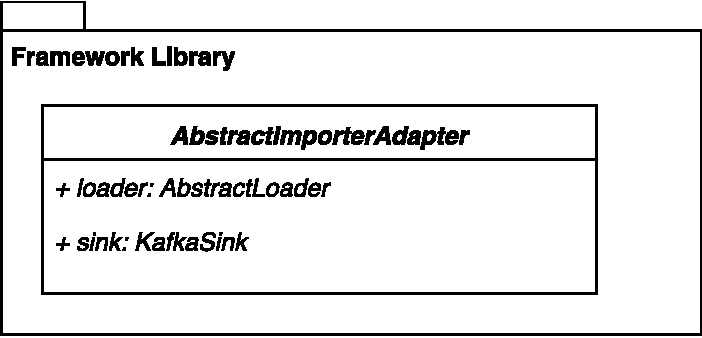
\includegraphics[width=0.4\textwidth]{import-adapter}\\
  \caption{Class diagram of input adapter sink and implementation}
  \label{fig:import-adapter}
\end{figure}

\subsection{Evaluation on library on recipe example}
The library for the import adapter is tested and showcased on the example of two sources of recipes. One source is a MongoDB collection \footnote{A collection in a MongoDB is equivalent to a table in a SQL database and contains a certain type of entities, called documents.}, the other source is a CSV file. Both sources contain recipes in a different schema. The input adapter library needs to be extend by a CSV loader. The extension is equal to the MongoDB source explained in section \ref{ssec:loadercomponent}, whereas the Alpakka source for CSV files is utilized. Concrete implementations of the both schemas as well s the raw recipe format are made and require very low programming work. The concrete implementation of the \textit{AbstractKafkaSink} only needs to provide a serializer for the global raw recipe. The utilization of the play-json\footnote{https://www.playframework.com/documentation/2.6.x/ScalaJson} library reduced the work to a minimum though a straight forward implementation of deserializers and serializers. The final importer job for both sources is a minimalistic implementation combining respectively the source and the common raw recipe Kafka sink.

\section{Implementation of the transformation pipeline}

The concept of the transformation pipeline suggests a component that can apply several transformation functions on raw entities of a deterministic schema and finally produces a generalized entity.

\subsection{Implementation of the common functionality}

The container framework Akka streams already provides a wide toolset of functionalities for data stream processing. As of the strong customization of transformation steps a less generic approach is chosen compared to the input adapters. 
\\\\
The main common component for the transformation pipeline are the input and output interfaces. Unifying the framework to one common data transportation layer and the concept of raw formats enables the reuse of components from the input adapter. Similar to the concept of the loader in the previous section a Kafka source is is implemented as part of the library for the transformation pipeline. The Kafka source is generic in that way that it is able to load any entity from a Kafka topic. The concrete implementation must then only provide a deserializer\footnote{A deserializer is a component, that defines how a class and its attributes are written to a specific output format.} for a concrete raw entity and the topic name.
\\\\
The component writing to the source, again Kafka, can be taken from the input adapter library classes. As outlined above, it is an generic implementation, that is able to write any object to a Kafka topic by providing a deserializer and the topic name.

\subsection{Implementation of transformation pipeline steps}

Having the source and sink for the transformation pipeline provided by the library, the connecting transformation steps can be introduced. For the realization of the stepwise approach we take advantage of the board toolset of Akka streams. The concept in chapter \ref{cha:chapter4} already explains idea of UDFs and the usage for the transformation pipeline. Mainly two functions of Akka streams are necessary to build the required pipeline. Those are \textit{map(.)} and \textit{mapAsync(.)}. The implementation of the pipeline is based on a concatenation of those two function where each step takes the element to prepare, performs a transformation and finally returns an modified or updated version of it. \textit{mapAsync(.)} has the additional benefit to call an external blocking resource without blocking the entire transformation pipeline. 
\\\\
A concrete implementation example that deals with raw recipe entities and transforms them to recipe entities is presented in the listening \ref{lst:pipeline}. It shows the transformation pipeline containing steps for preparation and parsing ingredients, instructions and image URLs. The source code of the individual functions is due to unimportance not listed here.

\begin{lstlisting}[style=myScalastyle,label={lst:pipeline},caption={Example transformation pipeline for raw recipes to recipes}]
val rawRecipeSource = KafkaRawRecipeSource("raw-recipes")
val recipeSink = KafakRecipeSink("recipes")

rawRecipeSource
  .map(ingredientService.processIngredients)
  .mapAsync(ingredientService.mapIngredients(_, 4, "de"))
  .map(processInstructions)
  .map(processServes)
  .map(createRecipe)
  .to(recipeSink)
\end{lstlisting}

\noindent The preparation and parsing steps in this concrete minimal example utilize the following technologies:
\\\\
\textbf{Regular expressions:}
The degree of automation of the feature extraction pipeline can be controlled by the effectiveness of applied transformation and parsing functions. Simple errors and deviations within the raw entity can be captured with regular expressions. Such a processing step is applied by calling \textit{ingredientService.processServes($\cdot$)}. It uses regular expressions that separate the field \textit{amount\_unit}. In this case a very deterministic input can be expected. Hence, a simple expression that matches on a combination of numbers and alphanumeric characters separated by zero or more spaces is sufficient. The capturing groups\footnote{A capturing group is a group of regular expressions that capture the text matched within that group as a unit.} for amount and unit enable a deterministic separation of both attributes for a given ingredient.
\\\\
\textbf{Self learning systems:}
As defined in the concept, the framework for feature extraction must also be able to learn from its input. This core requirement can easily applied in a further transformation function and the degree of learning defined by the implementing instance. An approach taken at the reference implementation of food recipes utilizes a full-text search engine and a continuous update of a learning data set for an increasing learning rate over time. 
\\\\
The implemented example of the framework uses Elasticsearch\cite{elasticsearch_2017} overcome the varying manifestations of ingredient names on recipes. Elasticsearch is a search engine based on the Apache Lucene\footnote{https://lucene.apache.org/core/} project. The search engine supports full-text search on schema-free JSON denouements powered by inverted indices\footnote{An inverted index is a lookup table where the alphabet of all possible words is listed and point to the documents in which they are contained.}. The idea is to find find the universal ingredient name by searching such with the raw ingredient string from the data source. A fuzzy\footnote{A fuzzy search on Elasticsearch finds all possible matches within a maximum edit distance.} search based on n-grams\footnote{A n-gram is a continuous sequence of substrings of length n of a underlying longer string (e.g. "reci", "ecip", "cipe" are all possible 4-grams for the string "recipe").} returns possible mappings of the raw ingredient string to universal ingredient names. 
\\\\
For example the string "Paprika, rot" will match the following universal ingredient names:
\begin{enumerate}
\item rote Paprika
\item Paprika
\item edelsüßes Paprikapulver
\end{enumerate}

This mapping can be taken and verified in a downstream quality assurance check. After a positive feedback the raw ingredient string (here "Paprika, rot") is stored with the ingredient Paprika as additional manifestation. Over time the data set contains several manifestations of one ingredient and enables better and more accurate search results. Over the long term the systems knowledge base is a list of ingredient documents containing the universal name and possible different wordings for each ingredient. The performance of the system is discussed in chapter \ref{cha:chapter6}.

\section{Implementation of output adapter}

The concept from section \ref{sec:componentsoutput} defines a component that provides the possibility of using several output formats. Figure \ref{fig:output-adapter} illustrates three different output adapters:
\begin{itemize}
\item Feature extractor
\item JSON serializer
\item Log appender
\end{itemize}

\begin{figure}[htb]
  \centering
  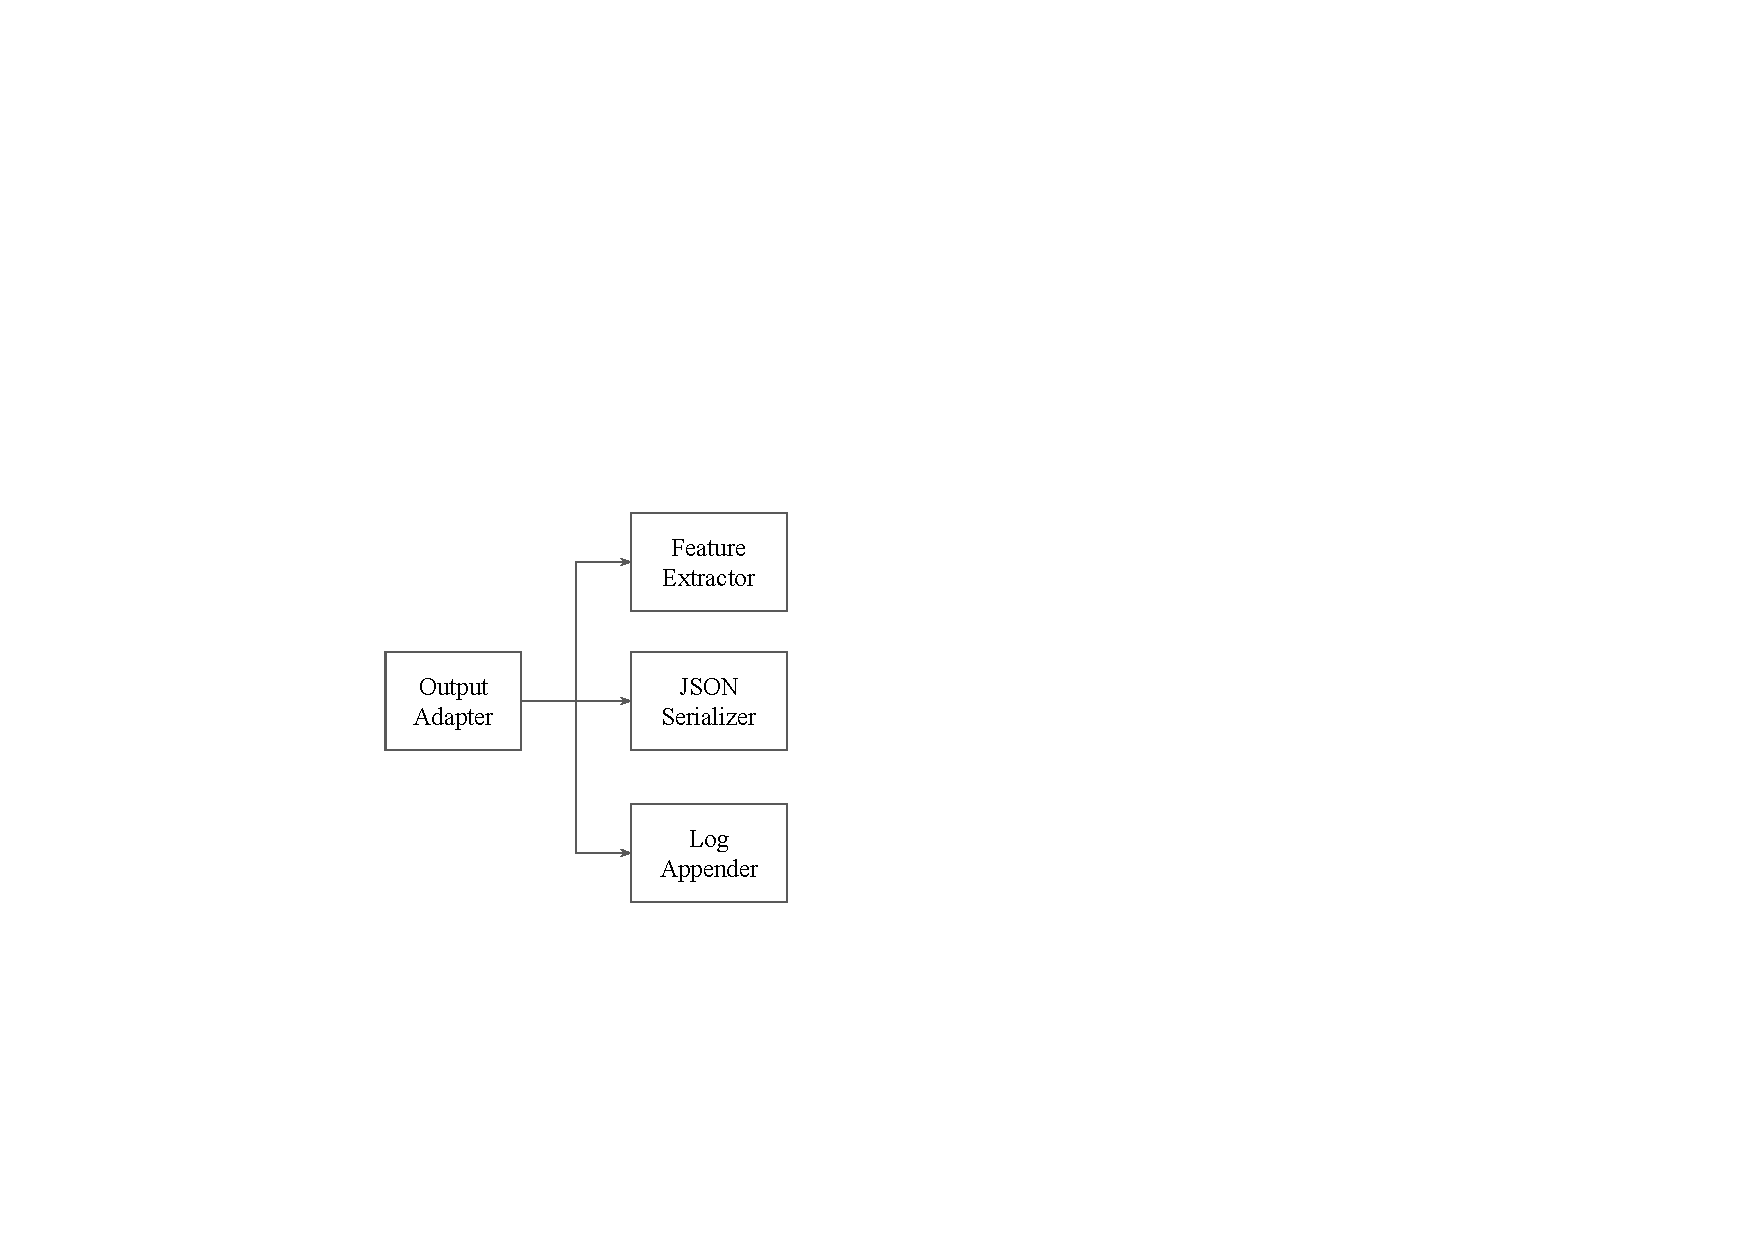
\includegraphics[width=0.4\textwidth]{output-adapter}\\
  \caption{Overview of message flow in the output adapter}
  \label{fig:output-adapter}
\end{figure}

The most important output adapter for a framework for automated feature extraction is clearly a feature extractor. The two further examples serve the visualization purpose. In the proof of concept implements the JSON serializer adapter is used for deliver the homogenized data for a quality assurance fronted. The Log appender is used for streaming the processed data into a standardized logging system, such as Logstash\footnote{Logstash is processing pipeline for bundling logs. See https://www.elastic.co/products/logstash}. 
\\\\
The overall adaptability was achieved by the Akka streams API. With Akka streams data streams can be built combined and spitted. For the output adapter the latter feature was used. Via simple DSL\footnote{Domain-specific language is a abstraction of a programming language for a specific domain} flow graphs of Akka streams can be set up. The listening \ref{lst:output} below. shows a reference implementation splitting one input source stream into three outgoing steams. The DSL of Akka streams is very intuitive and perfectly suitable for such a use case. It causes low programming overhead and promises fast exchange and extension of the adapter component. The source is again a Akka stream source reading from the underlying transportation layer. \textit{RecipeKafkaSource} only has do define the deserializer for the specific entity and the Kafka topic name of recipes.

\begin{lstlisting}[style=myScalastyle,label={lst:output},caption={Example of akka streams graph DSL for splitting streams}]
val in = RecipeKafkaSource("recipes")

val adapter = builder.add(Broadcast[Recipe](3))

val featureExtractorSink = RecipeFeatureExtractorSink()
val jsonSink = JsonSink[Recipe]()
val logAppenderSink = LogAppenderSink[Recipe]()

in ~> adapter ~> featureExtractorSink
        adapter ~> jsonSink
        adapter ~> logAppenderSink
\end{lstlisting}

The \textit{RecipeFeatureExtractorSink} finally creates feature vectors from a cleaned and stable recipe information entity. It is up to the demand of the developer which features are extracted. As feature engineering is not part of this work, details are not discussed here. The literature provides several approaches and techniques about feature engineering\cite{mastering_feature_engineering_2017} \cite{liu_2001}. 
\\\\
For the reference implementation binary features of the recipe ingredients were extracted. A binary feature vector is a vector only containing zeros and ones. If a specific attribute is present in the entity to represent, the corresponding field is set to one, otherwise to zero. Here the ingredients are used as features. The unified ingredient names are hashed to determine the the index within the the feature vector. This approach is reliable, as first, the possible manifestations of universal ingredients is finite, and second, the used hashing algorithm, here murmur-hash, returns a deterministic hash for each possible string. To reduce sparsity of the resulting feature vector most common ingredients and most uncommon ingredients where removed. A TF-IDF was used to achieve this. The term frequency - inverse document frequency is used in feature extraction to find significant features. For reference see the above provided literature.

\begin{figure}[htb]
  \centering
  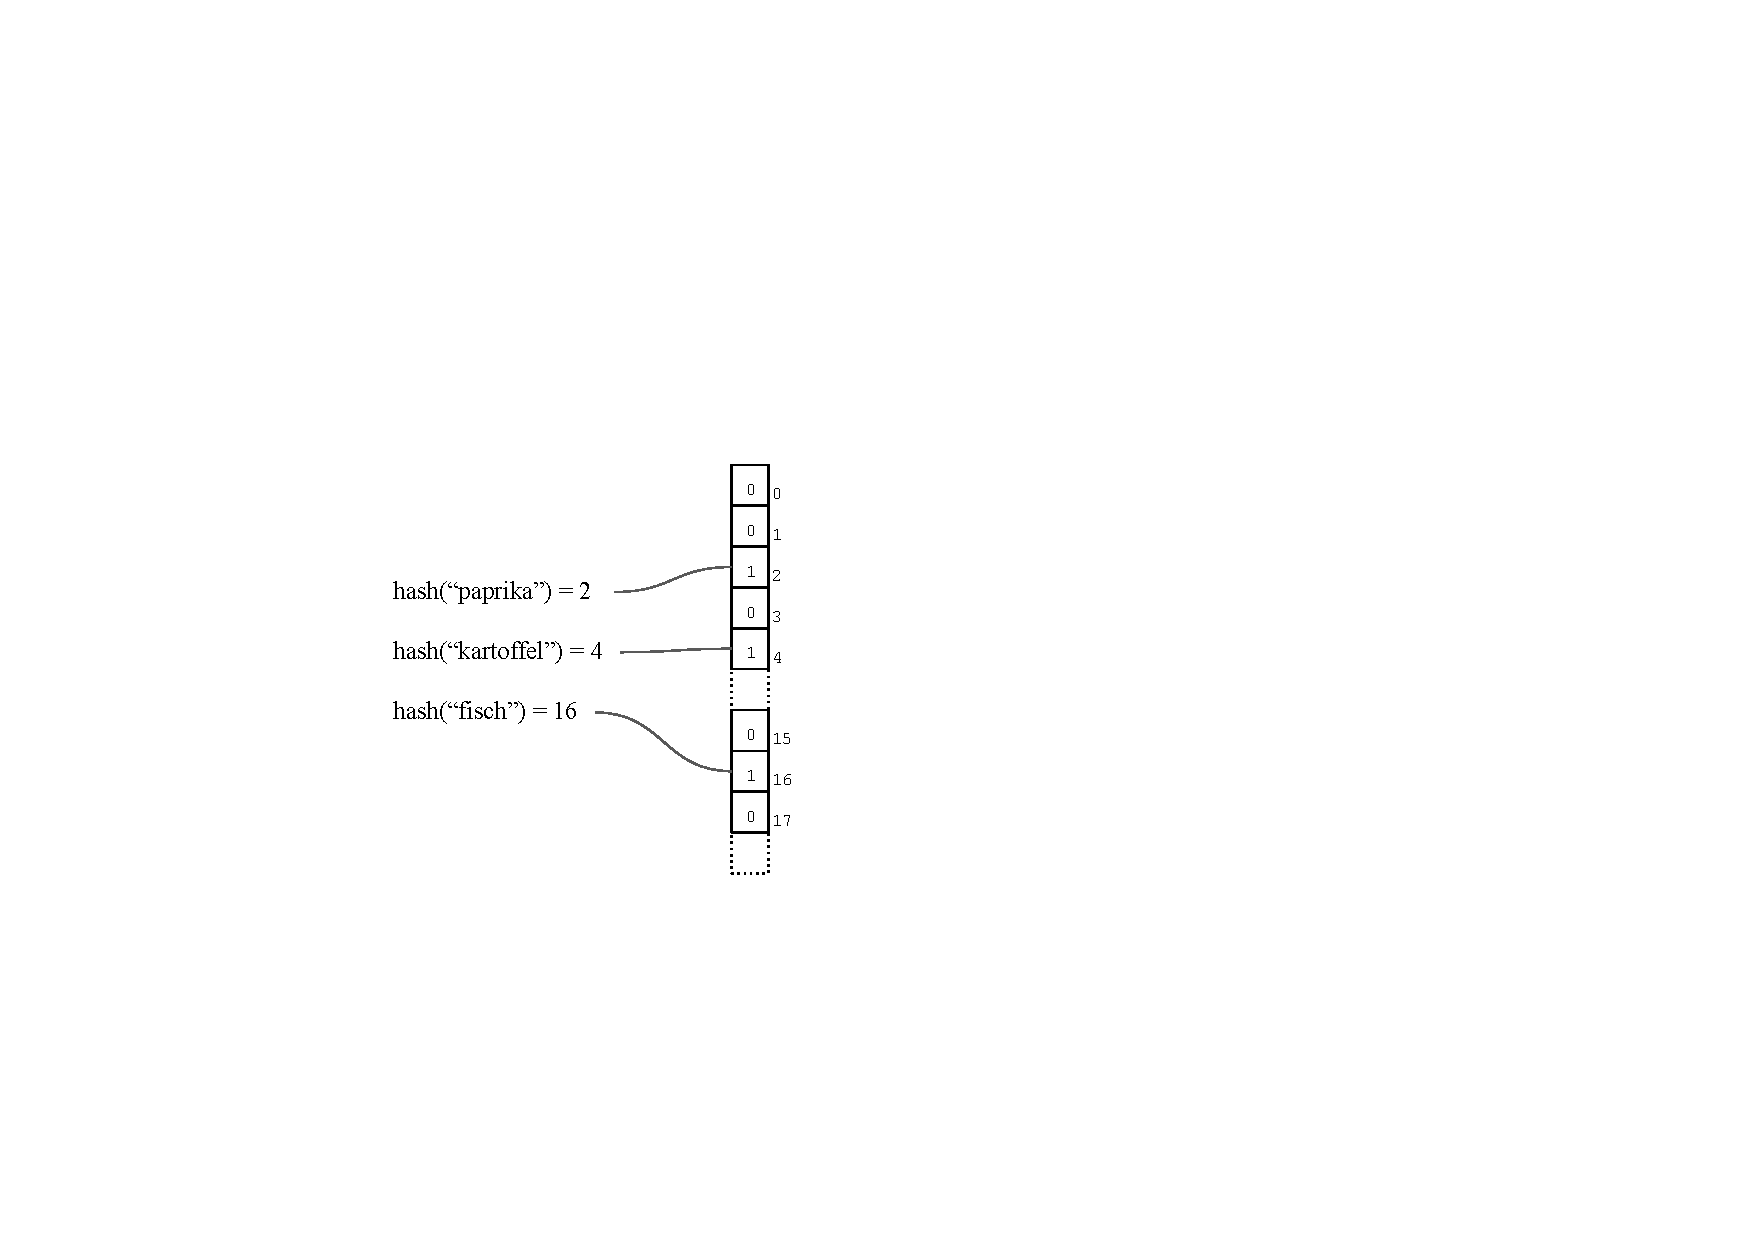
\includegraphics[width=0.4\textwidth]{bin-feature}\\
  \caption{Binary feature vector for the ingredients: paprika, kartoffel and fisch}
  \label{fig:bin-feature}
\end{figure}

Concluding it can be said, that the choice of the underlying container framework Akka streams and Kafka as well as the programming language Scala plays well together with the domain of automated data preparation. The available libraries and the introduced custom library reduced the implementation overhead for a processing pipeline for unification of semi-structured data. The idea of an additional abstraction layer on top of the data transfer component, Kafka and the Akka streams framework enables a simple adaption of the concrete framework implementation for different sources, entities and domains.

\section{Implementation of a quality assurance and error handling interface}

The quality of the out coming data is critical. Several aspects about that are discussed in the previous chapters. From an implementation point of view, the quality assurance can be considered as further step in the transformation pipeline. To be more accurate the quality assurance step must be the finalizing step before the data are send to the output adapter and features are extracted.
\\\\
As the implementation of an graphical user interface for quality assurance and administrative purposes is a very work and time costly project, only the data interface and the applicability within the suggested framework is given. 
\\\\
In the concrete case, this means that particular data are run through the quality assurance step. Whether an entity needs to be checked or not can be determined automatically. For instance if the regular expression on the field \textit{serves} does not apply. As in the ingredient mapping step only suggestions of the self learning system are given, in the concrete implementation every entity runs through a finalizing manual check. This can be reduced in future if learning system produces more reliable suggestions. The implementation for the quality interface sees a additional Kafka topic. After the transformation pipeline the entities are written to a dedicated quality assurance topic. The quality assurance application fetches the data from there, review is done and the entities are written back to new Kafka topic. From there the output adapter fetches the quality assured entities and features are extracted subsequently.

    \chapter{Evaluation\label{cha:chapter6}}

In this chapter the implementation of the automated feature extraction pipeline is evaluated. The re-usability and adaptability to different data sources outlined in the previous chapter is summarized and the applicability of the proposed framework assessed. Additionally we evaluate the quality of the out coming data, the quality assurance on code level as well as the scalability on throughput basis. 

\section{Applicability of the proposed framework concept}

The most evidence of applicability is given by the reference implementation outlined in detail in the previous chapter. This proof of concept shows that an stepwise approach of data homogenization and a final feature extraction is a solid concept. Providing a generalized library that can be utilized for different semi-structured information entities and in different domains increases the performance up to a high degree of automation for data unification. The framework allows to be extended on demand by further data sources, parsing steps or output adapters as defined in the requirements of chapter \ref{cha:chapter3}. The next chapter will give a general conclusion about the proposed framework.

\section{Performance Measurements\label{sec:performance}}

Measuring the performance of the overall implementation is restricted due to the absence of an reference dataset. Depending on the desired quality of out coming data, which relates to the kind of features finally used, the quality requirements vary. 
\\\\
A more interesting an measurable index is the performance of single processing steps within the parsing pipeline. See figure \ref{fig:basicconcept} as reference. 
\\\\
For the evaluation of the learnability of the system a toy dataset is created and the performance of automated data cleansing by using a full-text search engine is evaluated. The toy dataset contained roughly 300 universal ingredients. Those where manually extracted from a dataset of circa 200 recipes and indexed\footnote{The process of loading documents in to Elasticsearch during which the inverted index is build internally.} using n-grams (specifically 3-grams up to 20-grams) in a local Elasticsearch setup. Raw ingredient strings extracted from the publicly available recipe section of the Kaufland website are used to verify the accuracy on hit rate. For evaluation of the performance more than 200 ingredients from Kaufland where manually mapped to the universal ingredient. 
\\\\
The performance is measured by averaging the index of the true value within the scored Elasticsearch search result. Meaning the cost of a miss increases linearly wit the distance to the top scored result. The search result is upper bounded by 15 results and the cost of of a not found element fixed by 16.  For instance when matching the raw ingredient \textit{"Paprika, rot}, the universal ingredient \textit{"rote Paprika"} occurs on index 3 of the result list, 3 is considered as the cost of the miss match. If \textit{"rote Paprika"} is not contained in the result list, 16 is set as the cost. The sum of all costs is averaged across test examples.
\\\\
On the initial run using 200 labeled ingredients and the above descried setup a average score of 1.83 was reached. This meas that the average offset from the top of the result list was less than 1. For comparison, if half on the universal ingredient is on index one, and half of the ingredient on index two, a average of 1.5 results. considering the fact, that the set of universal ingredients exceeds size of the toy dataset, 300, by far, this are very promising initial results. 

A second run on an updated Elastic search index definitions, increased the average score by 20\%. Using 2-grams instead of 3-grams as the lower-bound for the ingredient index resulted in a average score of 1.74. This can be explained by the fact, that ingredients with 2 character names in German exists. Those are ignored by a index only using 3 or more grams.

In a third run the toy dataset was extend in a way, such that each of the universal ingredient had exactly one further manifestation. Rerunning the performance evaluation as set up in the second run lead to an average score of 1.67. This number is the perfect prove for the learnability of the proposed feature extraction framework.

\section{Test Environment\label{sec:testenvir}}

Independent testing of components is a major aspect in software quality. The library components of the proposed framework where unit tested using the official scala-test framework. \textit{WordSpec} provides an very intuitive and human readable setup of tests on code level. Those assure the stability of the library on updates, bug fixes and implementation of further features. \\\\
The system is very strongly connected to different database systems. The functioning of the different connectors, not only to the underlying data transfer layer also to data sources as MongoDB and the learning system with Elastic search must be ensured after maintenance work. 

The independence of the system from actual running instances of the named databases is very important when it comes to automatized testing. The common approach to achieve the independence is the usage of embedded versions of the required database systems. Open source libraries for an embedded Kafka, embedded Elasticsearch and embedded MongoDB are used for unit and integration tests of the framework implementation.

% https://github.com/manub/scalatest-embedded-kafka
% https://github.com/allegro/embedded-elasticsearch
% https://github.com/flapdoodle-oss/de.flapdoodle.embed.mongo

\section{Scalability\label{sec:scal}}

\subsection{Scalability on domain level}

The extendability of the provided library is a great win for unifying data across several sources. This is mainly possible through the quick extension of input adapters as well as the stepwise approach of parsing data. The introduction of raw entities gives space for input adapters to add more sources, as well as stability to the downstream parsing logic on the other hand. The pre-generalization of data plays a significant role in the flexible approach of the framework and the developed concept of it.
\\\\
An re-usage of the scope in this work created framework and its concrete implementation in the domain of food products showed that is possible to scale the framework over further domains. This is enabled by the abstraction of data problems on a meta level. The domain specifics can be realized on a higher level ob abstraction which does not interfere with the concept of the framework itself.

\subsection{Scalability on data throughput level}

The introduction of this work gives insights of about the novel amount of data available nowadays. The choice of the container framework in section \ref{sec:env} pointed out that from this work of perspective not requirement for a technical scalability is defined. Having said this, it is also important to say that the proposed framework and the stated concept does indeed support the technical scaling. This is mainly thank to the chosen underlying transportation layer, Kafka. As Kafka is applicable in distributed systems and the framework on top of it is designed such that the data for each information entity to be parsed lives in a different topic, the application can simply be scaled by adding additional parsing nodes running the same application.
\\\\
The concept describes the abstraction of the framework implementation of the container framework, as well as the data transpiration layer. If the demand for an highly distributed data parsing and feature extraction system arises, the proposed framework can be easily ported to frameworks like Apache Flink or Apache Spark. The concrete implementation of the UDFs are simple map functions which can be simply ported to different systems.
















    \chapter{Conclusion\label{cha:chapter7}}

The final chapter summarizes the overall work and the approach of this thesis of finding an suggestion for a framework that enables automated feature extraction on semi-structured data. A conclusion about the suggested framework is made, encountered problems are discussed and a future outlook is given.  

\section{Summary\label{sec:summary}}

Working with heterogeneous data requires knowledge about their nature. Analyzing the development of data storage over the last centuries gives deep insights and helps to understand the underlying problem. It gives a clear image about the common patterns used in different environments and systems, for instance the approach of SQL versus no SQL. The common understanding promotes the ability of generalizing the stated problem in chapter \ref{cha:chapter1}. Splitting up the data diversity into different categories leads to a straight forward but structured approach of dedicated solution finding. The categorization of entity level problems and attribute level problems in chapter \ref{cha:chapter2} helped to develop the two-step approach the framework applies finally. The abstraction of format problems, and varying schema problems shows again in the generic approach of the concept of the input adapter.
\\\\
Enriching a data stream processing engine with the ability of automated data parsing shows as a performing concept. Data processing frameworks nowadays provide a established tool set and a stable environment to extend them by custom libraries and finally build domain specific applications. A functional approach proofed to be the right choice in the domain of data processing and data parsing. The framework and its implementation unifies perfectly with available open source technologies. 
\\\\
\noindent The work done can be summarized into the following work steps

\begin{itemize}
\item Analysis of underlying data storage technologies
\item Derivation of data problems and categorization of those
\item Assessment of data problem categories
\item Requirement engineering for a framework being able to handle formulated problems
\item Concept design based on problem statements and requirements
\item Implementation and evaluation of the concept in consideration of the defined requirements
\end{itemize}

\section{Problems Encountered\label{sec:problems}}

Mainly only problems with malformed data are encountered. This is mainly handled by the implemented requirement of a processing guarantee, but finally does not vanish the need of manual rework. Not all problems can be solved by adjusting the parsing pipeline. At this point is it to mention that the costs of malformed data is up to final use case of the environment the framework is operating in. The choice between or applying manual work for introducing the corrected version of the data into the downstream system or discarding un-processable data has to be made. The frameworks design and the set up concept still allows both options. 

\section{Outlook\label{sec:outlook}}

Future work will raise the degree of automation of the implementation of the proposed framework. Concrete ideas and concepts are already in place to enrich the framework with machine learning techniques. More specifically speaking, a draft of extending the parsing pipeline by predictive component for data normalization is submitted. This will help to archive a higher degree of automation and minimize the usage of error prone static components.
\\\\

Concluding it can be said, that the suggested framework can handle 

% ---------------------------------------------------------------
\backmatter % no page numbering from here
    \addchap{List of Acronyms}

\begin{tabbing}
spacespacespace \= space \kill
JSON	 \> 	Javascript Object Notation	 \\
XML	 \> 	Extensible Markup Language	 \\
UDF	 \> 	User Defined Function	 \\
SQL	 \> 	Structured Query Language	 \\
noSQL	 \> 	not only SQL	 \\

\end{tabbing}
\endinput

		
    % if you want to provide a glossary with explanations of important terms put it in here

    \bibliographystyle{geralpha}
    \bibliography{./bib/bibliography}
    
    %\addchap{Annex}

\begin{appendix}

\lstset{language=,caption=Sourcecode Listing,captionpos=b,
label=yahoowidgetkon,showstringspaces=false,
basicstyle={\fontfamily{pcr}\selectfont\footnotesize}}
\begin{lstlisting}
<?xml version="1.0" encoding="UTF-8"?>
<widget>
	 <debug>off</debug>
	 <window name="myWindow" title="Hello Widget" visible="true">
		 <height>120</height>
		 <width>320</width>
		 <image src="Resources/orangebg.png">
			<name>orangebg</name>
			<hOffset>0</hOffset>
			<vOffset>0</vOffset>
		</image>
		 <text>
			 <name>myText</name>
			 <data>Hello Widget</data>
			 <color>#000000</color>
			 <size>20</size>
			 <vOffset>50</vOffset>
			 <hOffset>120</hOffset>
		 </text>
	</window>
</widget>
\end{lstlisting}

\newpage


\lstset{caption=SIP request and response packet\cite{SIPBook},
captionpos=b,label=sippacket,showstringspaces=false,
basicstyle={\fontfamily{pcr}\selectfont\footnotesize}}
\begin{lstlisting}
INVITE sip:bob@network.org SIP/2.0
Via: SIP/2.0/UDP 100.101.102.103:5060;branch=z9hG4bKmp17a
Max-Forwards: 70
To: Bob <sip:bob@network.org>
From: Alice <sip:alice@ims-network.org>;tag=42
Call-ID: 10@100.101.102.103
CSeq: 1 INVITE
Subject: How are you?
Contact: <sip:xyz@network.org>
Content-Type: application/sdp
Content-Length: 159
v=0
o=alice 2890844526 2890844526 IN IP4 100.101.102.103
s=Phone Call
t=0 0
c=IN IP4 100.101.102.103
m=audio 49170 RTP/AVP 0
a=rtpmap:0 PCMU/8000

SIP/2.0 200 OK
Via: SIP/2.0/UDP proxy.network.org:5060;branch=z9hG4bK83842.1
;received=100.101.102.105
Via: SIP/2.0/UDP 100.101.102.103:5060;branch=z9hG4bKmp17a
To: Bob <sip:bob@network.org>;tag=314159
From: Alice <sip:alice@network.org>;tag=42
Call-ID: 10@100.101.102.103
CSeq: 1 INVITE
Contact: <sip:foo@network.org>
Content-Type: application/sdp
Content-Length: 159
v=0
o=bob 2890844526 2890844526 IN IP4 200.201.202.203
s=Phone Call
c=IN IP4 200.201.202.203
t=0 0
m=audio 49172 RTP/AVP 0
a=rtpmap:0 PCMU/8000
\end{lstlisting}


\end{appendix}

\endinput


\end{document}